%% ergebnisse.tex

\chapter{Ergebnisse und Diskussion}
\label{ch:Ergebnisse}

\section{Allgemeine Merkmale des Netzwerkes}
\label{sec:result-allg-merkm-des}

\section{Eigenschaften einzelner Schl\"ussel}
\label{sec:result-key-properties}

\section{Zusammenhangskomponenten und Communities}
\label{sec:result-zusamm-und-comm}

\section{Struktur der starken Zusammenhangskomponenten}
\label{sec:result-komponentenstruktur}

\begin{figure}[t]
  \centering
  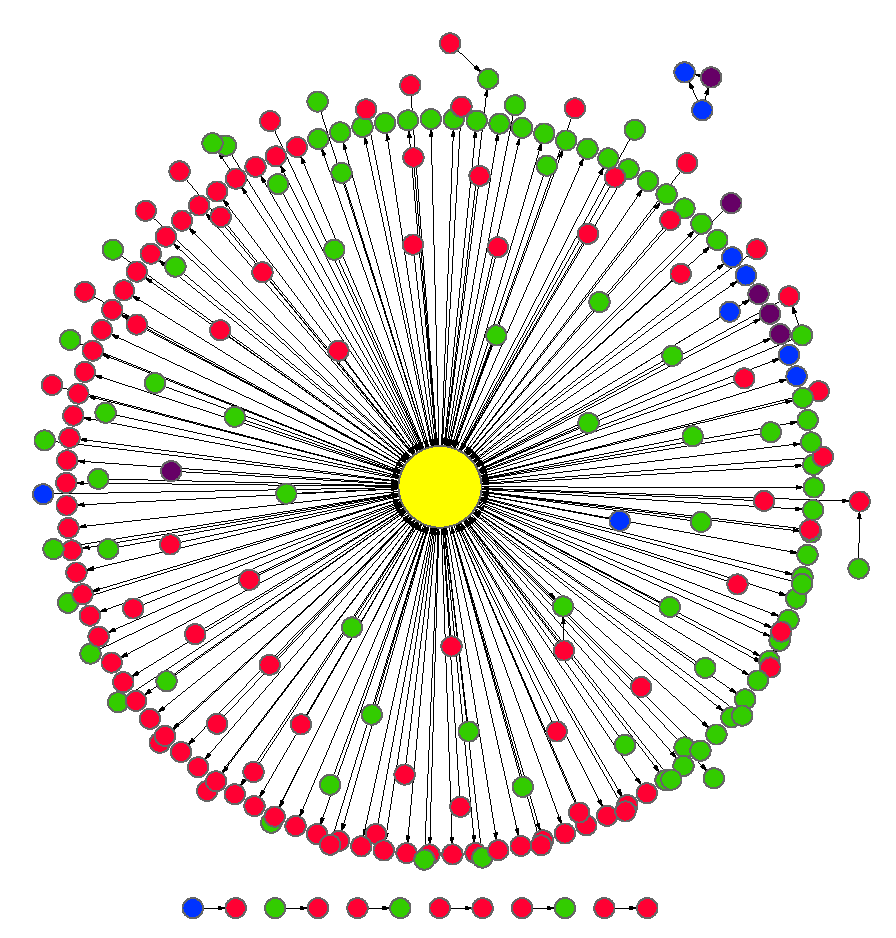
\includegraphics[scale=1.0]{images/component-metagraph-8.pdf}
  \caption{Struktur der starken Zusammenhangskomponenten bis zur
    Grösse 6 (rot = Grösse 6-10, grün = Grösse 11-20, blau = Grösse
    21-30, violett = Grösse $>= 31$, gelb = MSCC)}
  \label{fig:komponenten-struktur}
\end{figure}

Foobar bla bla bla.

\subsection{Communities}
\label{sec:result-communities}

Die Zerlegung des gerichteten Graphen mit dem Algorithmus von Rosval
et al. lieferte keine verwertbaren Ergebnisse. Zwar wurde eine
Zerlegung in 2869 Partitionen berechnet. Allerdings gilt f\"ur die
grosse Mehrzahl dieser Knotenmengen, dass der durch sie induzierte
Teilgraph \"uberhaupt keine Kanten hat. Nur f\"ur ca. 160 Partitionen
hat der jeweils induzierte Teilgraph Kanten, in allen F\"allen
allerdings sehr wenige (zwischen 1 und 104 f\"ur eine Partition der
Gr\"osse 682). Dass die Knoten einer Partition in allen F\"allen so
gut wie keine interne Vernetzung haben und damit der Definition von
Communities absolut nicht entsprechen, ist ein klarer Hinweis, dass
die berechnete Zerlegung die tats\"achliche modulare Struktur des
Graphen nicht sinnvoll wiedergibt. Dass der Graph in der Tat eine
ausgepr\"agte modulare Struktur hat, zeigen die anhand des
ungerichteten Graphen berechneten Zerlegungen, die auch unter
inhaltlichen Gesichtspunkten Sinn ergeben. Diese Struktur kann sich
auch nicht erst durch die Reduzierung des gerichteten auf einen
ungerichteten Graphen ergeben. Die berechnete Zerlegung mit etlichen
grossen Partitionen ohne interne Vernetzung ist in keinem Fall ein
sinnvolles Ergebnis eines Community-Algorithmus und spricht daher
f\"ur eine fehlerhafte Berechnung. Ob diese allerdings auf Fehler in
der verwendeten Implementierung der Autoren
\footnote{http://www.tp.umu.se/~rosvall/code.html} oder auf Fehler im
Algorithmus zur\"uckgeht, ist nicht bekannt.

Die nichtdeterministische LP-Berechnung lieferte Modularity-Werte mit
einer maximalen Abweichung von 0,002. Hier wurde das Maximum
verwendet. F\"ur die COPRA-Berechnung ergaben sich mit steigender
maximaler \"Uberlappung $v$ nur bis $v\le 3$ steigende
Modularity-Werte, dar\"uber hinaus fielen sie konstant ab. Deshalb
wurde die Berechnung mit $v=3$ verwendet. Die dort berechneten
Modularity-Werte hatten eine geringe Standardabweichung von 0,003. 

\begin{figure}[t]
  \centering
  \subfloat[]{\label{fig:comsize-lp} 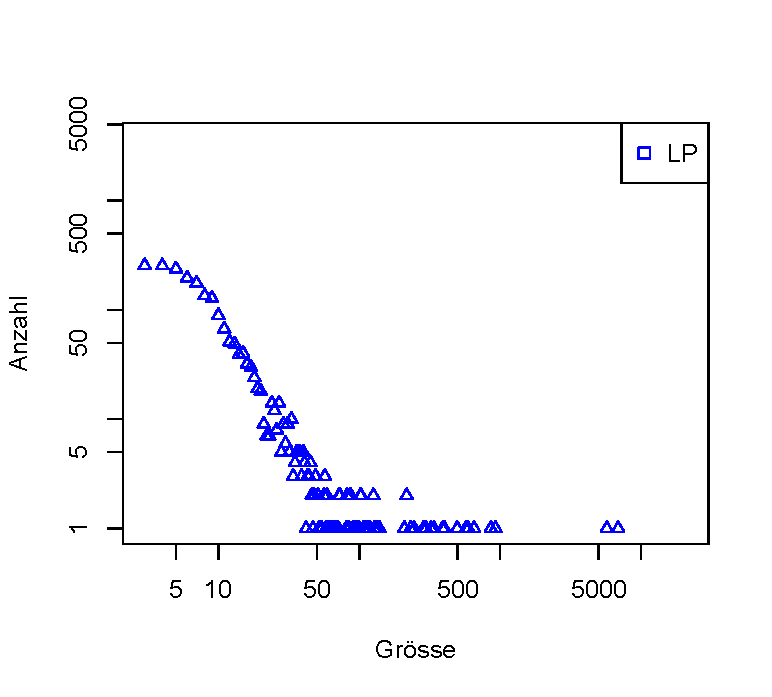
\includegraphics[scale=0.65]{images/community-size-dist_label.pdf}}
  \subfloat[]{\label{fig:comsize-bl2} 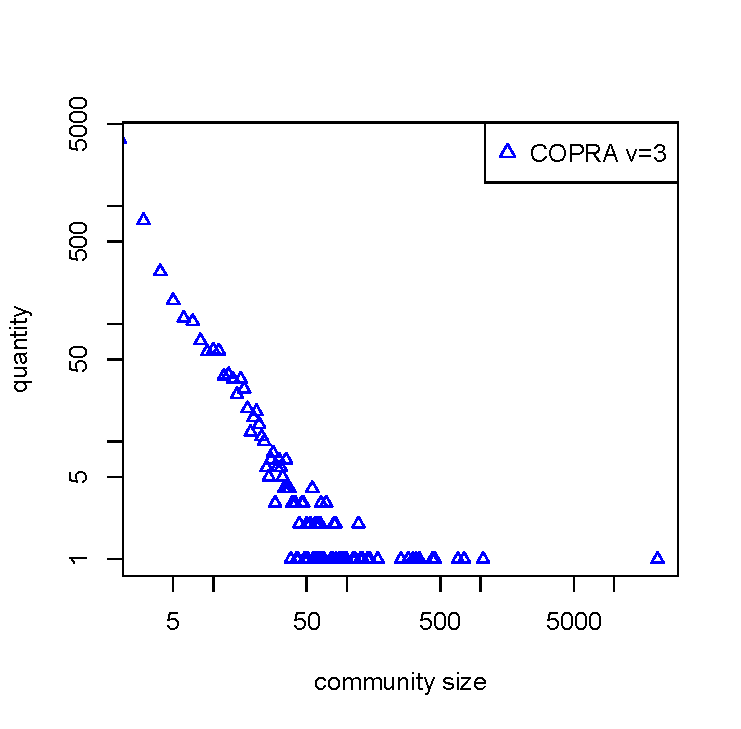
\includegraphics[scale=0.65]{images/community-size-dist_copra.pdf}}\\
  \subfloat[]{\label{fig:comsize-bl5} 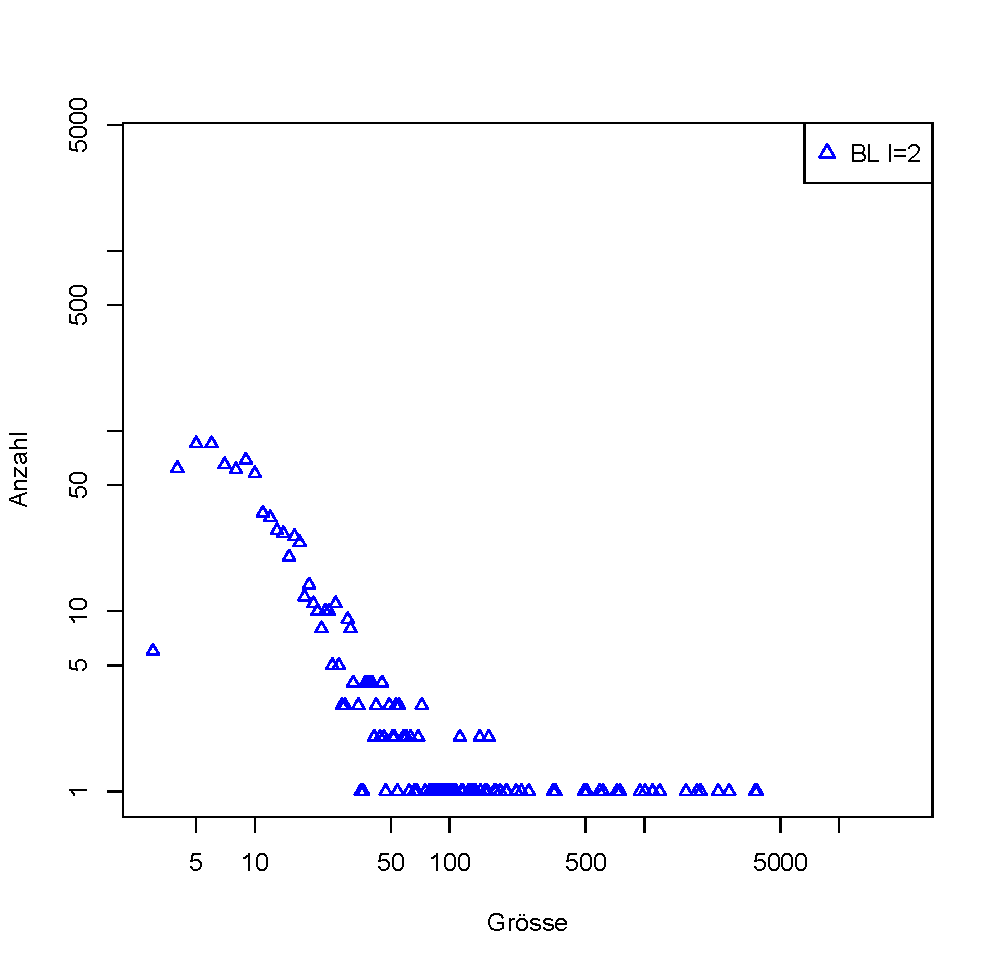
\includegraphics[scale=0.65]{images/community-size-dist_bl2.pdf}} 
  \subfloat[]{\label{fig:comsize-copra} 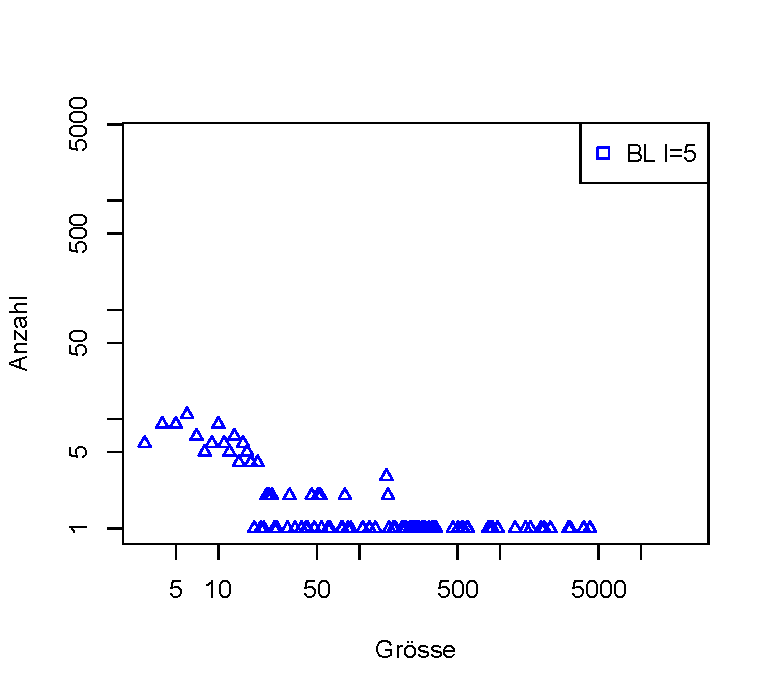
\includegraphics[scale=0.65]{images/community-size-dist_bl5.pdf}}
  \caption{Gr\"ossenverteilung der Communities}
  \label{fig:comsizedist}
\end{figure}


\begin{table}[h]
  \centering
  \footnotesize
  \begin{tabular}{l|c|c|c}
    Algorithmus & Modularity & Communities &
    Enthaltene Knoten \\
    \hline
    FM & 0,596 & 552 & foo \\
    LP & 0,658 & 1834 & foo \\
    BL ($l=2$)& 0,701 & 936 & foo \\
    BL ($l=5$)& 0,710 & 186 & foo \\
    COPRA & (0,786) & 1354 & foo
  \end{tabular}
  \caption{Modularity-Werte, Anzahl der Communities mit mehr als 3
    Knoten sowie die Anzahl der insgesamt in diesen Communities (>3) enthaltenen
    Knoten 
    f\"ur die Algorithmen Fast-Modularity (FM), Label-Propagation
    (LP), Blondel et al. (BL) auf Level 2 und 5 sowie COPRA. Der
    Modularity-Wert f\"ur COPRA entspricht der Modularity-Definition
    f\"ur \"uberlappende Zerlegungen nach \cite{Nicosia2009} und kann mit den anderen
    Werten nicht verglichen werden.}
  \label{tab:foo}
\end{table}

Der insgesamt recht hohe Modularity-Wert weist darauf hin, dass der
Graph in der Tat eine ausgepr\"agte modulare Struktur hat, wie dies
von einem sozialen Netzwerk erwartet wird.

\begin{table}[h]
  \centering
  \footnotesize
  \begin{tabular}{l|c|c|c|c|c}
    Algorithmus & TLD-S & TLD-M & SLD-S & SLD-M & SIG \\
    \hline
    FM & 293 (53\%) & 247 (44\%) & 66 (11\%) & 194 (35\%) & 128
    (23\%) \\
    \hline
    LP & 1048 (57\%) & 755 (41\%) & 277 (15\%) & 720 (39\%) &
    553 (30\%) \\
    \hline
    BL ($l=2$) & 499 (53\%) & 417 (45\%) & 41 (4\%) & 254 (27\%) & 26
    (14\%) \\
    \hline
    BL ($l=5$) & 85 (47\%) & 85 (47\%) & 15 (8\%) & 38 (21\%) & 26
    (14\%) \\
    \hline
    COPRA & 792 (58\%) & 525 (38\%) & 259 (19\%) & 533 (39\%) & 555 (40\%)

  \end{tabular}
  \caption{SLD-TLD-Zuweisung, TIME-CORR}
  \label{tab:assign}
\end{table}

Aus Tab. \ref{tab:assign} geht hervor, dass f\"ur alle Zerlegungen
fast alle Communities einer Top-Level-Domain zuordnenbar sind oder von
einer TLD dominiert werden. Werden die generischen Top-Level-Domains
(gTLD: com, org, net, info, ...) abgezogen, verbleiben im Fall von COPRA
noch 519 (38\%) Communities, die einer TLD (und damit einer
\emph{Country-Coded TLD (ccTLD)}) zugeordnet werden k\"onnen und 315
(23\%), die von einer ccTLD dominiert werden. F\"ur die anderen
Zerlegungen ergeben sich \"ahnliche Werte. Damit ist immerhin etwa die
H\"alfte der Communities einem Land zuordnenbar. F\"ur die von einer
gTLD dominierten Communities ergeben Stichproben, dass sich die
Teilnehmer der meisten dieser Communities anhand der Namen zumindest
einem Sprachraum zuweisen lassen.

Dieses Ergebnis ist naheliegend. Es wird davon ausgegangen, dass ein
wesentlicher Faktor, der das Zustandekommen von Signaturen
beeinflusst, die sozialen Kontakte einer Person sind. Es ist weiterhin
naheliegend, dass sich diese sozialen Kontakte unter anderem aufgrund
von Sprachbarrieren und der r\"aumlichen N\"ahe haupts\"achlich im
Rahmen eines Landes ergeben.

Zwar k\"onnte argumentiert werden, dass das Internet die geographische
bzw. nationale Beschr\"ankung sozialer Kontakte aufhebt. Allerdings
spielt die die geographische N\"ahe eine wichtige Rolle im
Signaturprozess. Die verbreitete Prozedur f\"ur das Signieren eines
Schl\"ussels setzt ein direktes pers\"onliches Treffen der
Signierenden voraus (siehe Abschnitt \ref{sec:sozi-komp-des}). Es ist
anzunehmen, dass die \"uberwiegende Mehrheit der PGP-Benutzer die
meiste Zeit in einem Land und damit in einem geographisch
eingegrenzten Bereich verbleibt. Damit kommen f\"ur diese Mehrheit
\"uberwiegend nur Bewohner des gleichen Landes als Signaturpartner in
Frage. Als Mechanismen f\"ur die internationale Vernetzung kommen dann
etwa internationale Konferenzen in Frage. Nur ein sehr kleiner Teil
der PGP-Benutzer d\"urfte die notwendige internationale Mobilit\"at
aufweisen, so dass sich seine Signaturen nicht \"uberwiegend einem
geographischen Bereich bzw. einem Land zuweisen lassen.

\begin{figure}[h]
  \centering
  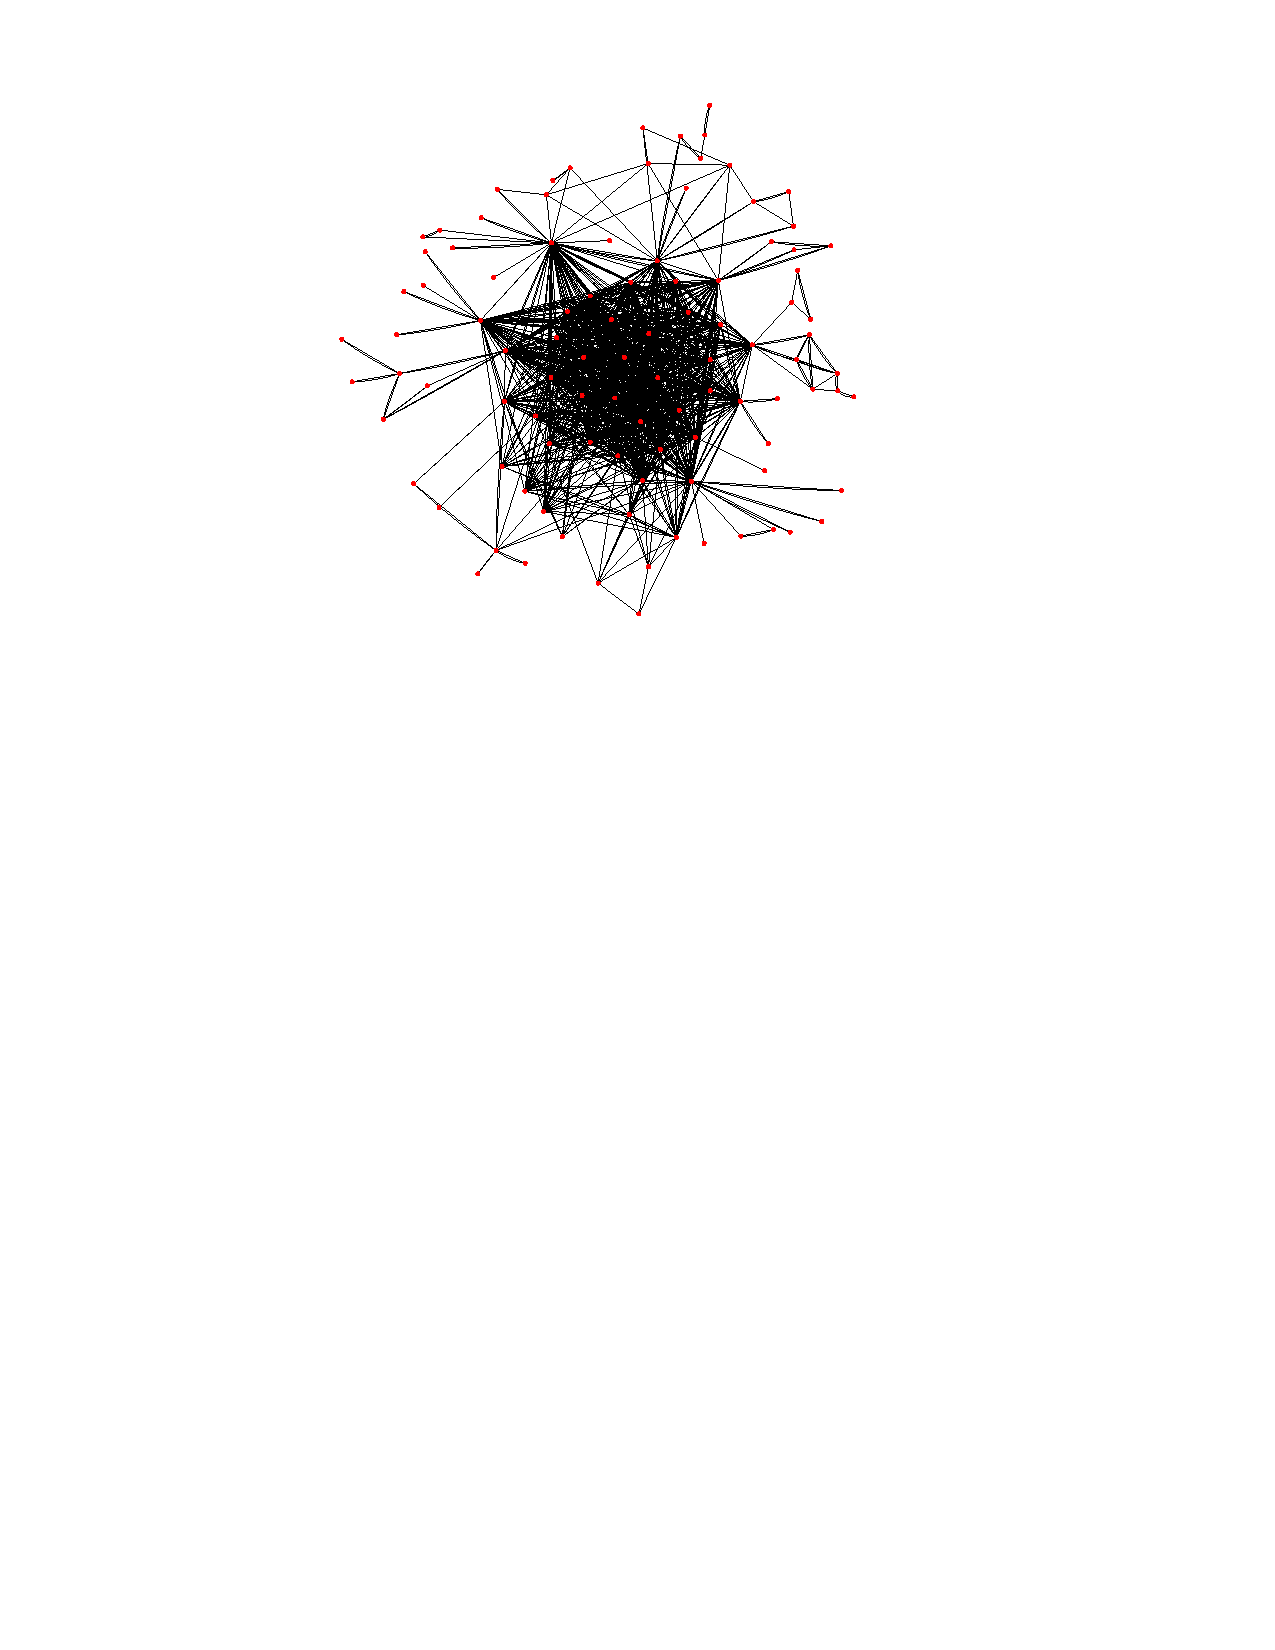
\includegraphics[scale=1.5]{images/subgraph-label-time-fa62cc57cd35e9f90b85435efc407ad5.pdf}
  \caption{Community mit zeitlicher Korrelation der Signaturen (LP,
    100 Knoten, 72\% der Signaturen innerhalb eines Monats)}
  \label{fig:time-corr-com-normal}
\end{figure}


\begin{figure}[h]
  \centering
  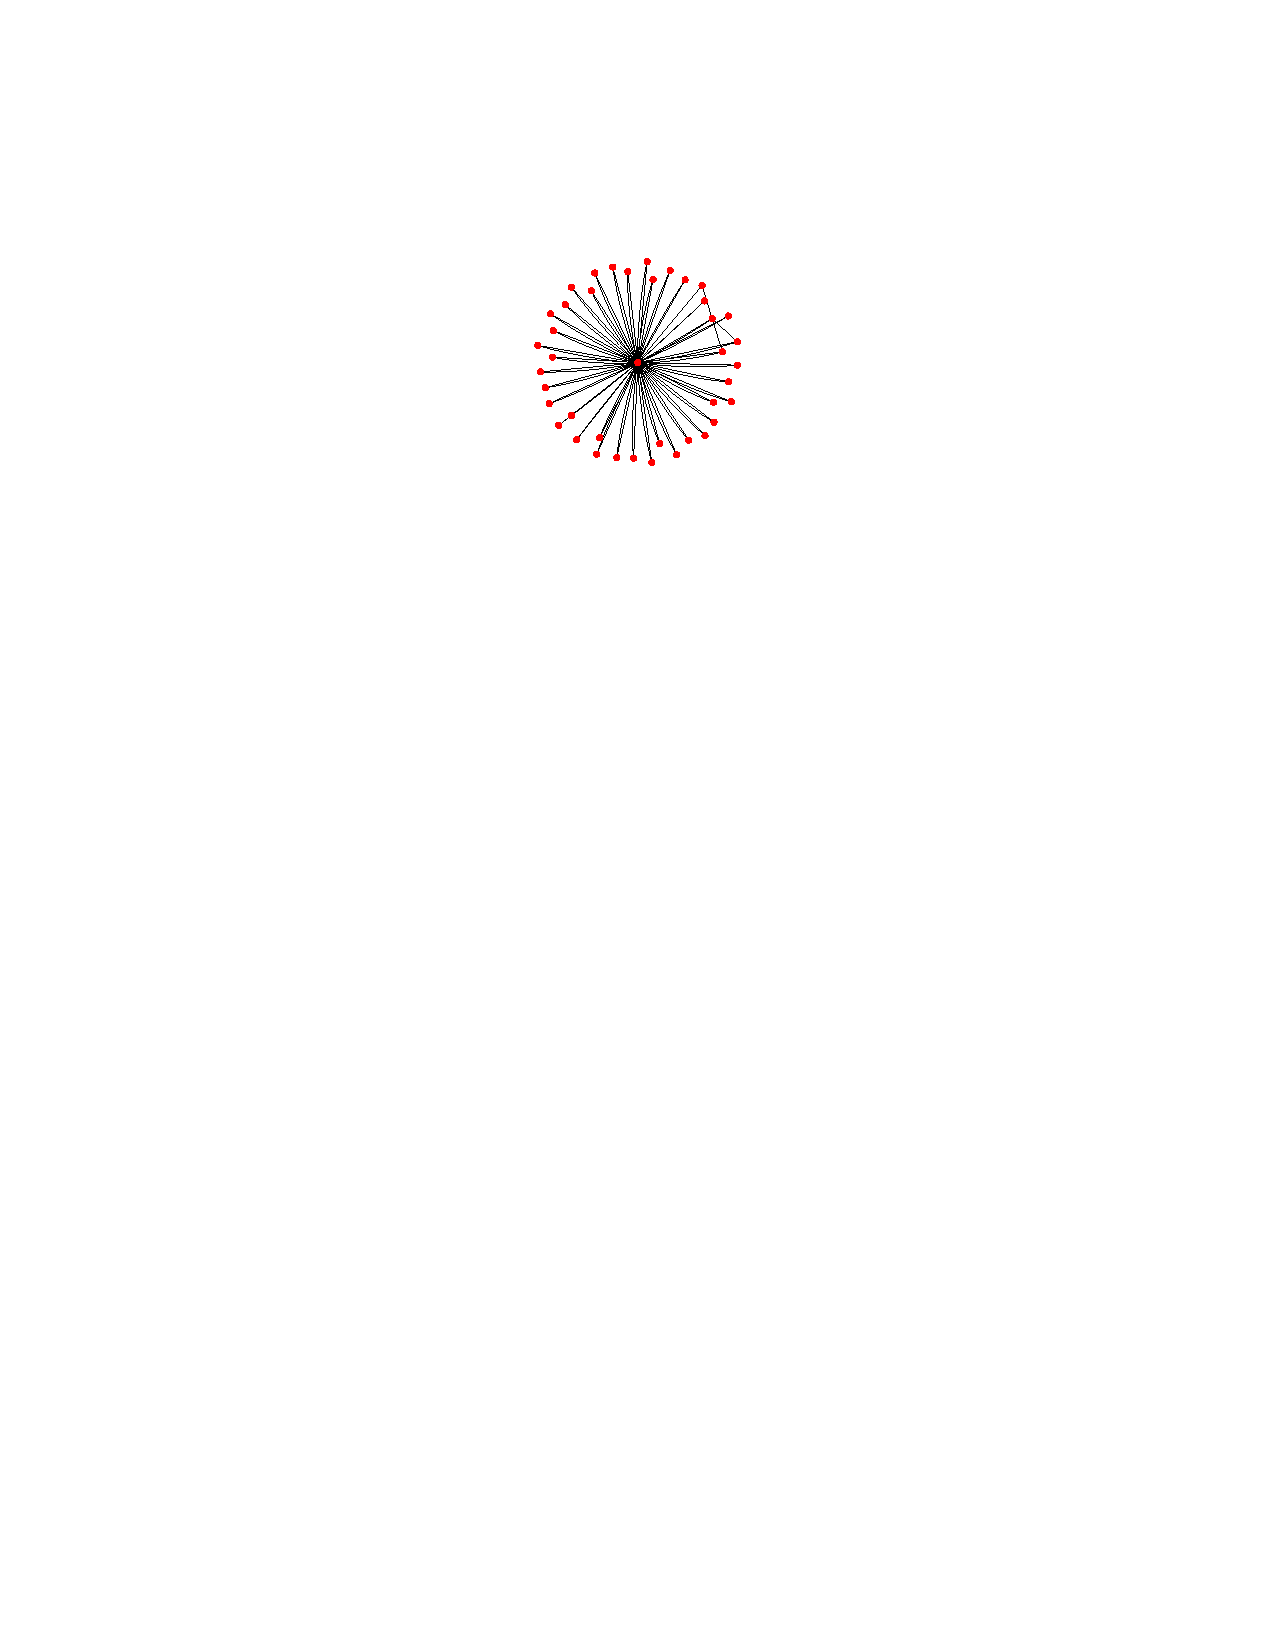
\includegraphics[scale=1.3]{images/label-subgraph-41-star-c222345bc5eb1f9eff80d58a81861974.pdf}
    \caption{Community mit zeitlicher Korrelation der Signaturen (LP,
      41 Knoten, 84 \% der Signaturen innerhalb eines Monats)}
  \label{fig:time-corr-com-star}
\end{figure}


Es stellt sich die Frage, ob die zeitliche Korrelation der Signaturen
in einer Community ein geeignetes Mittel ist, um Keysigning-Parties zu
erkennen. Neben dem zeitlichen Zusammenhang der Signaturen ist ein
weiteres Merkmal einer Keysigning-Party wie in
Ab. \ref{sec:sozi-komp-des} beschrieben, dass jeder Teilnehmer mit
(fast) jedem anderem Teilnehmer Signaturen austauscht, so dass sich
eine fast vollst\"andige Vermaschung -- fast eine Clique --
ergibt. Eine stichprobenartige Untersuchung in den Communities zeigt,
dass die meisten Communities mit zeitlicher Korrelation zumindest
teilweise dieses Merkmal zeigen. Abb. \ref{fig:time-corr-com-normal}
zeigt ein Beispiel einer solchen Community. Etwa die H\"alfte der
Knoten ist in einer Fast-Clique enthalten, deren Knoten mit (fast)
allen anderen vernetzt sind. Dieser innere Teil des Teilgraphen
entspricht genau dem Bild, das als Resultat einer Keysigning-Party
erwartet wird. Auch wenn dies auf die meisten der Communities mit
zeitlicher Korrelation zutrifft, gibt es auch
Gegenbeispiele. Abb. \ref{fig:time-corr-com-star} zeigt eine
Community, die zwar das Kriterium der zeitlichen Korrelation
erf\"ullt, ansonsten aber nichts mit dem erwarteten Bild einer KSP
gemein hat. Allerdings erf\"ullt der Teilgraph trotzdem das Kriterium
der Community, da die Knoten am Rand nur Signaturen zu dem zentralen
Knoten haben und damit die interne Kantendichte deutlich h\"oher ist
als die externe. Um solche Extremf\"alle auszuschliessen, ist als
zus\"atzliches Kriterium f\"ur die Erkennung von KSPs ein hoher
durchschnittlicher Grad der Knoten denkbar.


\begin{figure}[h]
  \centering
  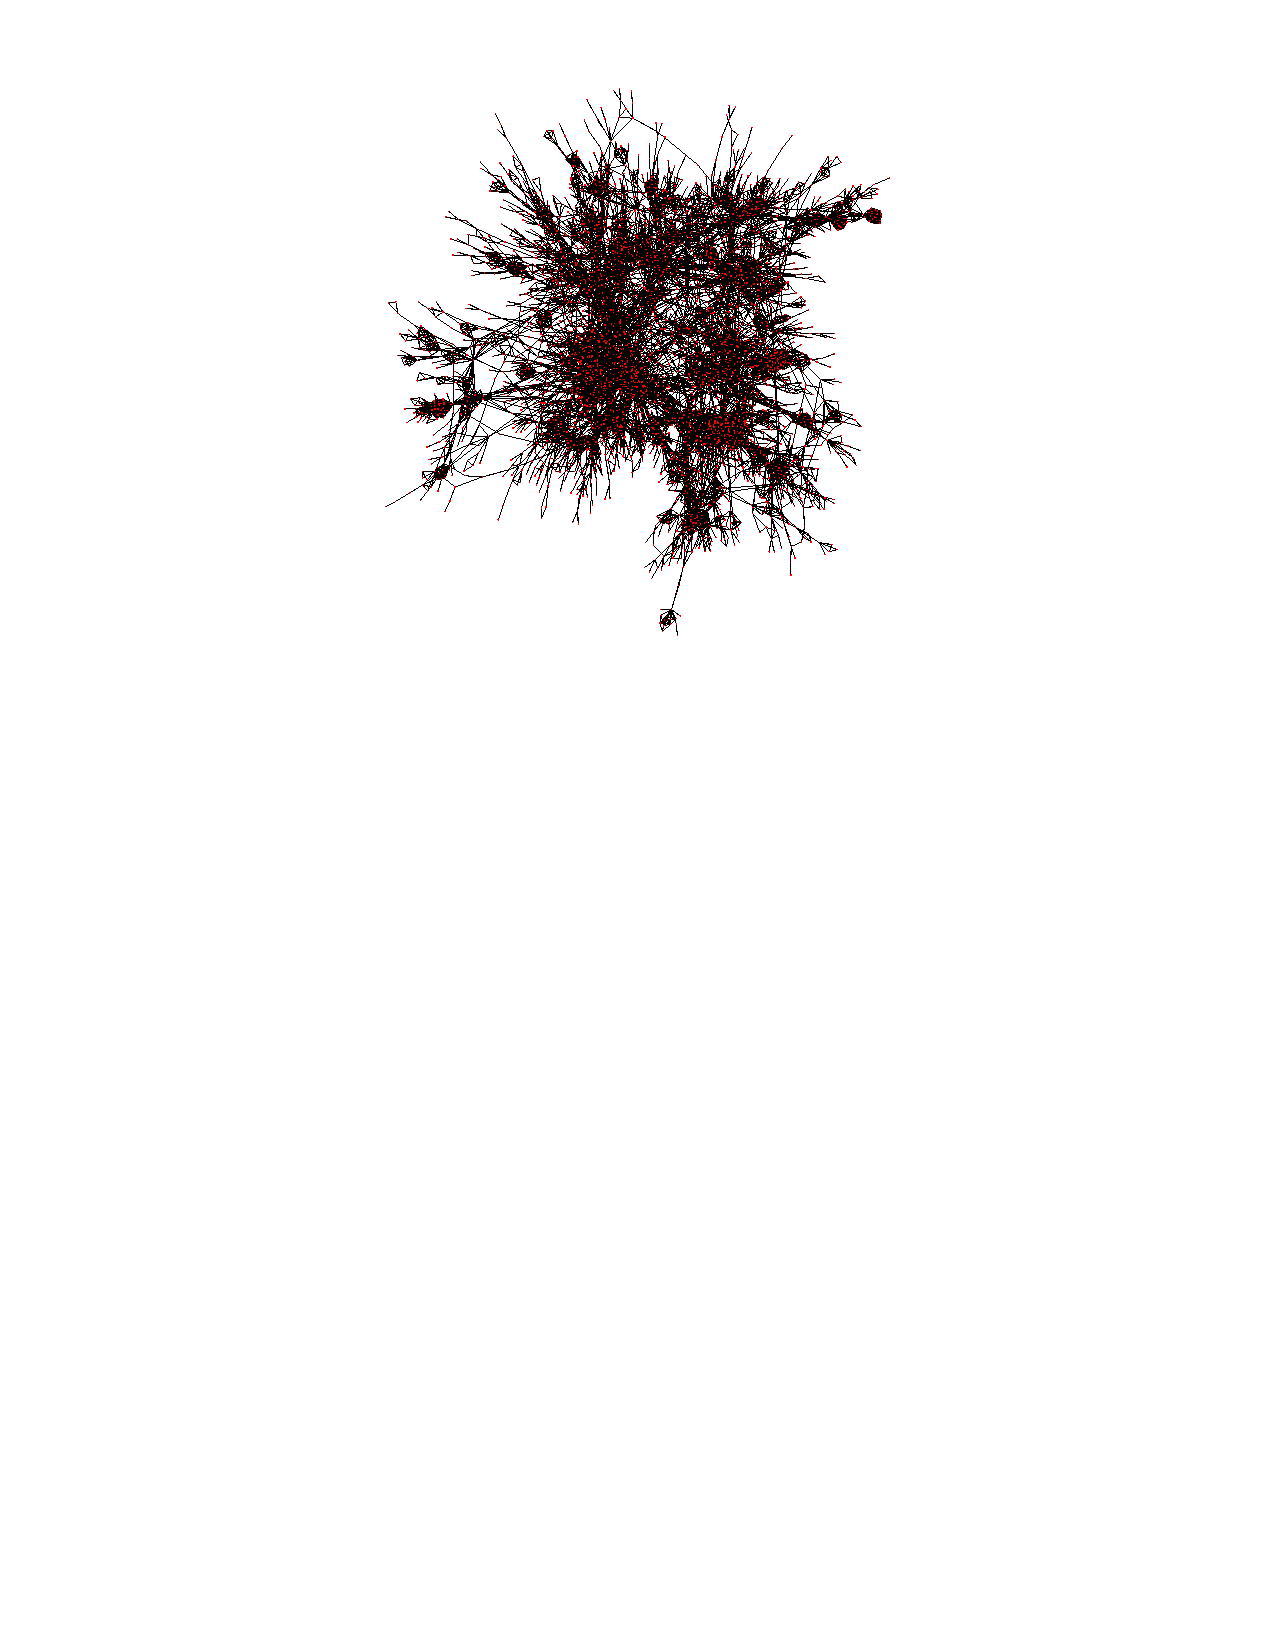
\includegraphics[scale=1.7]{images/fastmod-subgraph-large-modular-6525064ccab580a0b304a3620b197d7a.pdf}
  \caption{Grosse Community mit modularer Struktur (Berechnet mit
    Fast-Modularity, Force-directed layout)}
  \label{fig:large-community-modular}
\end{figure}

Communities k\"onnen sich nicht nur \"uberlappen. Genauso k\"onnen
einzelne Communities intern wieder eine modulare Struktur haben, so
dass sie sich in mehrere Communities zerlegen lassen.
Abb. \ref{fig:large-community-modular} illustriert, dass die
Verwendung von Methoden zur Berechnung \"uberlappender Communities
sinnvoll sein kann. In der Zeichnung des induzierten Teilgraphen einer
grossen Community (4767 Knoten) aus der
Fast-Modularity-Partitionierung sind etliche dicht gezeichnete
Zusammenballungen von Knoten zu sehen, die nur wenige Kanten nach
aussen haben. Diese k\"onnen als Community-artige Strukturen
interpretiert werden. Zwar kann argumentiert werden, dass die
Zeichnung die Struktur des Teilgraphen nicht notwendigerweise sinnvoll
wiedergibt, dass also die dichten Teilbereiche in der Zeichnung nur
Artefakte der Zeichenmethode darstellen. Allerdings zeigt Noack, dass
starke \"Ubereinstimmungen zwischen einer energieoptimalen Einbettung
eines Graphen in die Ebene nach der Force-directed-Methode und einer
Partitionierung eines Graphen mit optimaler Modularity bestehen
\cite{Noack2009}. Es scheint daher gerechtfertigt, eine Zeichnung
eines Graphen (Force-directed) mit markanten dichten Bereichen als
Indiz f\"ur eine modulare Struktur dieses Graphen zu betrachten.
\begin{figure}[h]
  \centering
  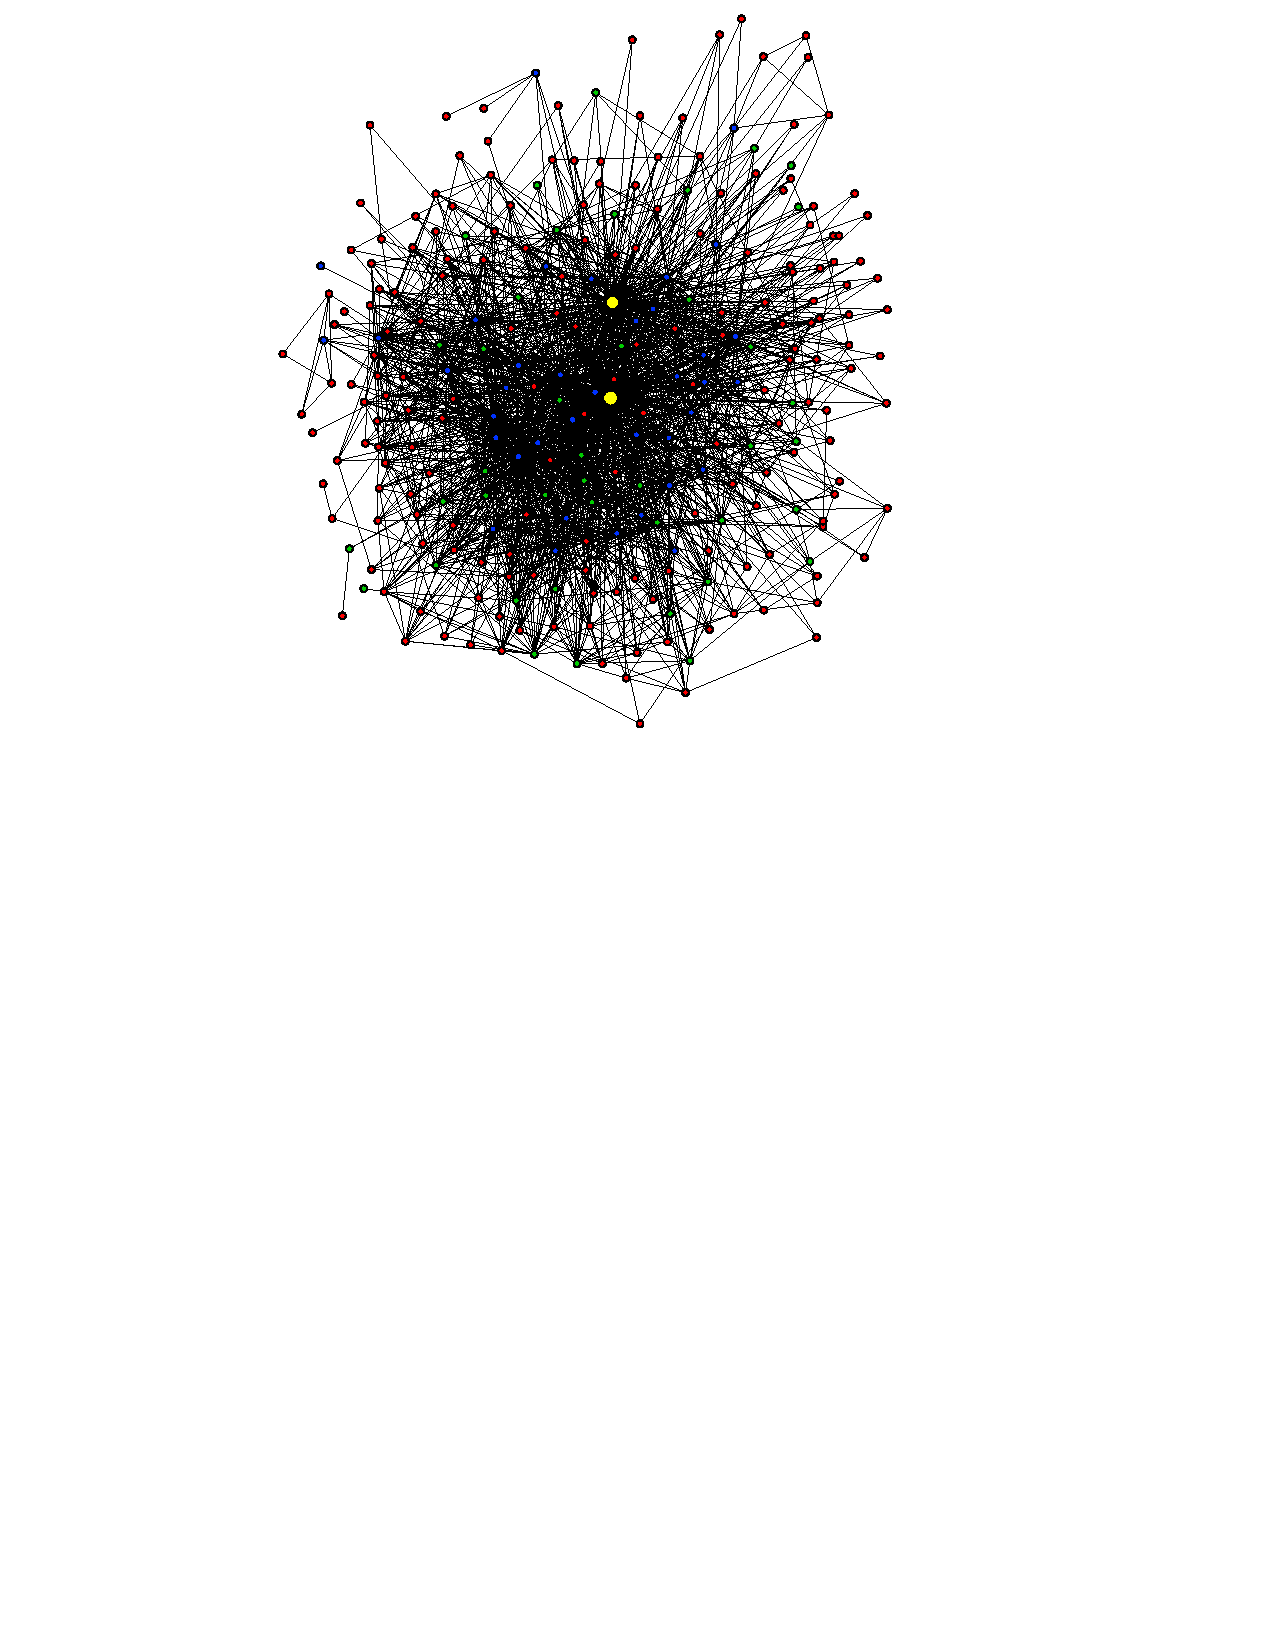
\includegraphics[scale=1.5]{images/label-prop-metagraph-20-narrow-cut.pdf}
  \caption{Struktur der Communities (Label-Propagation) (rot: Gr\"osse
    $<50$, gr\"un: Gr\"osse $<100$, blau: Gr\"osse < 1000, gelb:
    Gr\"osse > 1000).}
  \label{fig:metagraph-com-label}
\end{figure}


\begin{figure}[h]
  \centering
  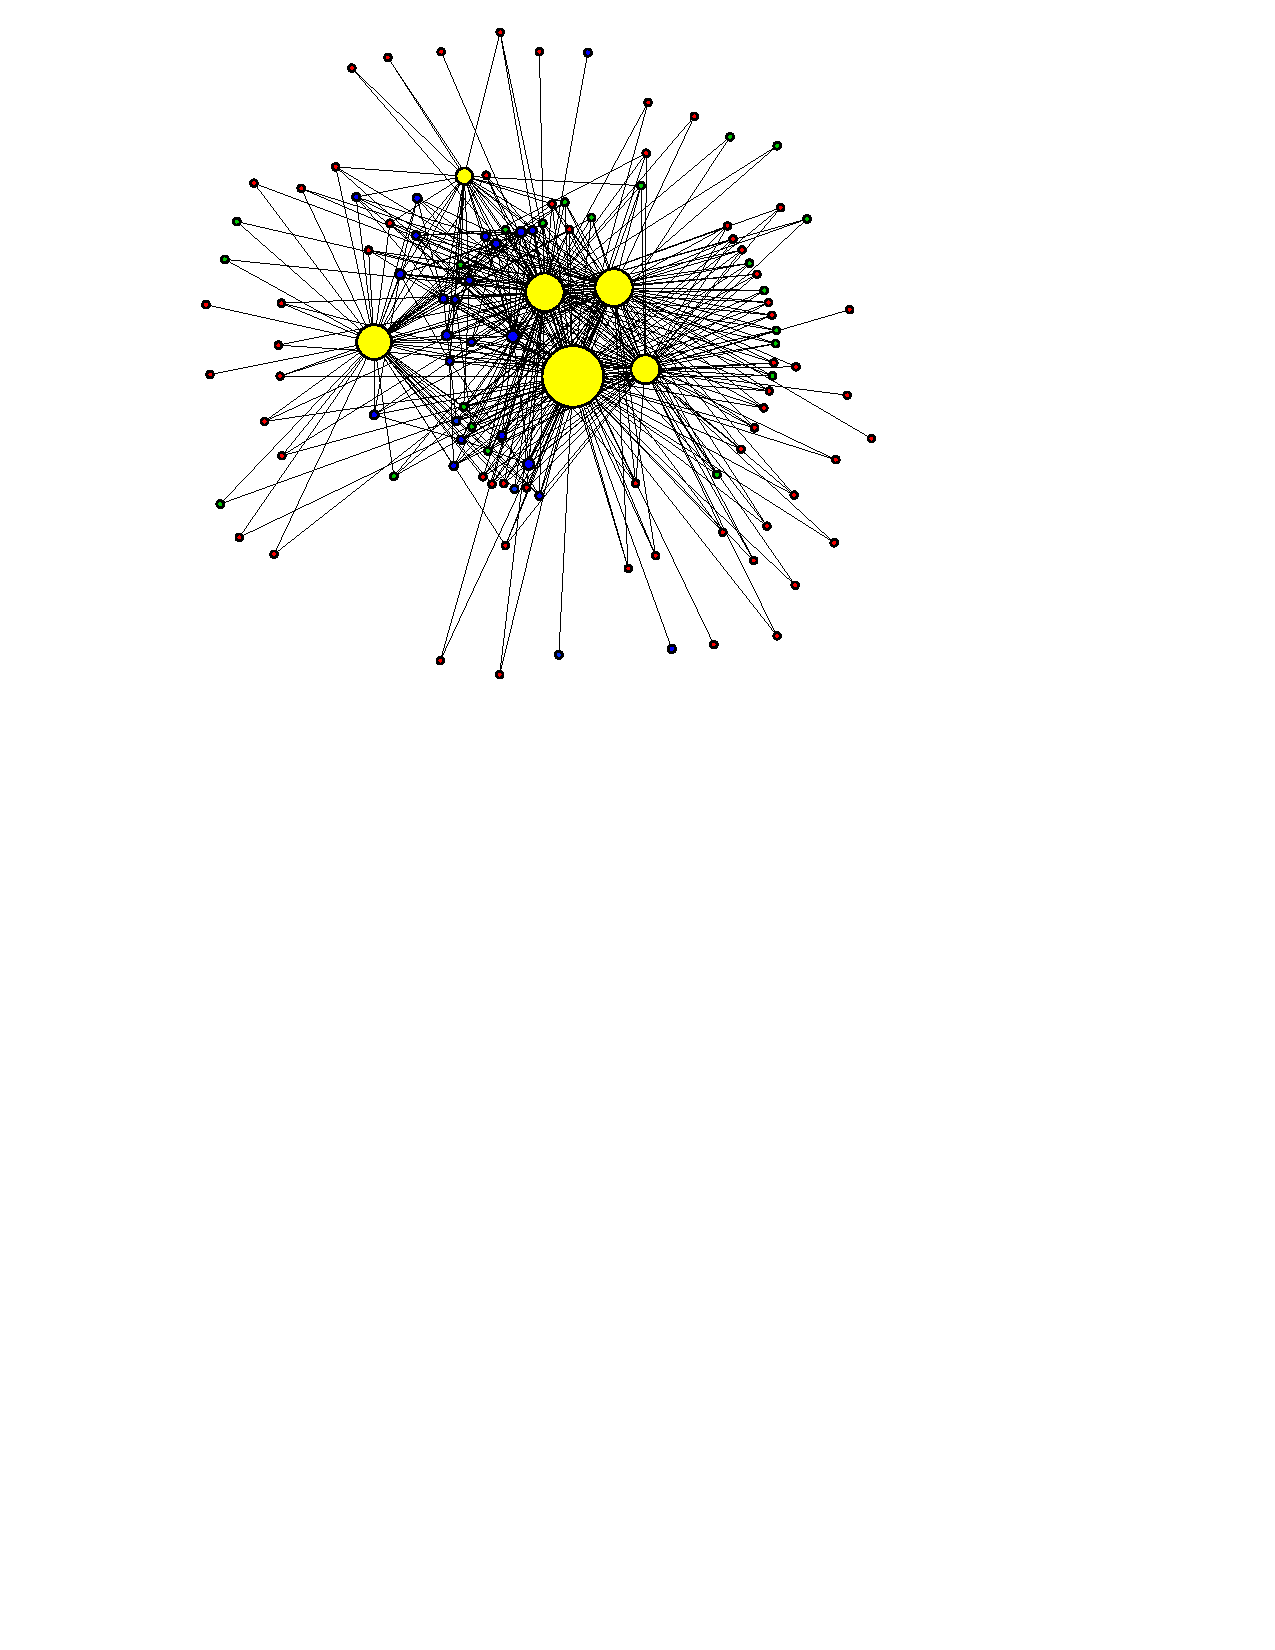
\includegraphics[scale=1.0]{images/fastmod-metagraph-20.pdf}
  \caption{Struktur der Communities (Fast Modularity) (Knotenf\"arbung
    wie in Abb.\ref{fig:metagraph-com-label})}
  \label{fig:metagraph-com-fastmod}
\end{figure}


\begin{figure}[t]
  \centering
  \subfloat[]{\label{fig:comsize-lp} 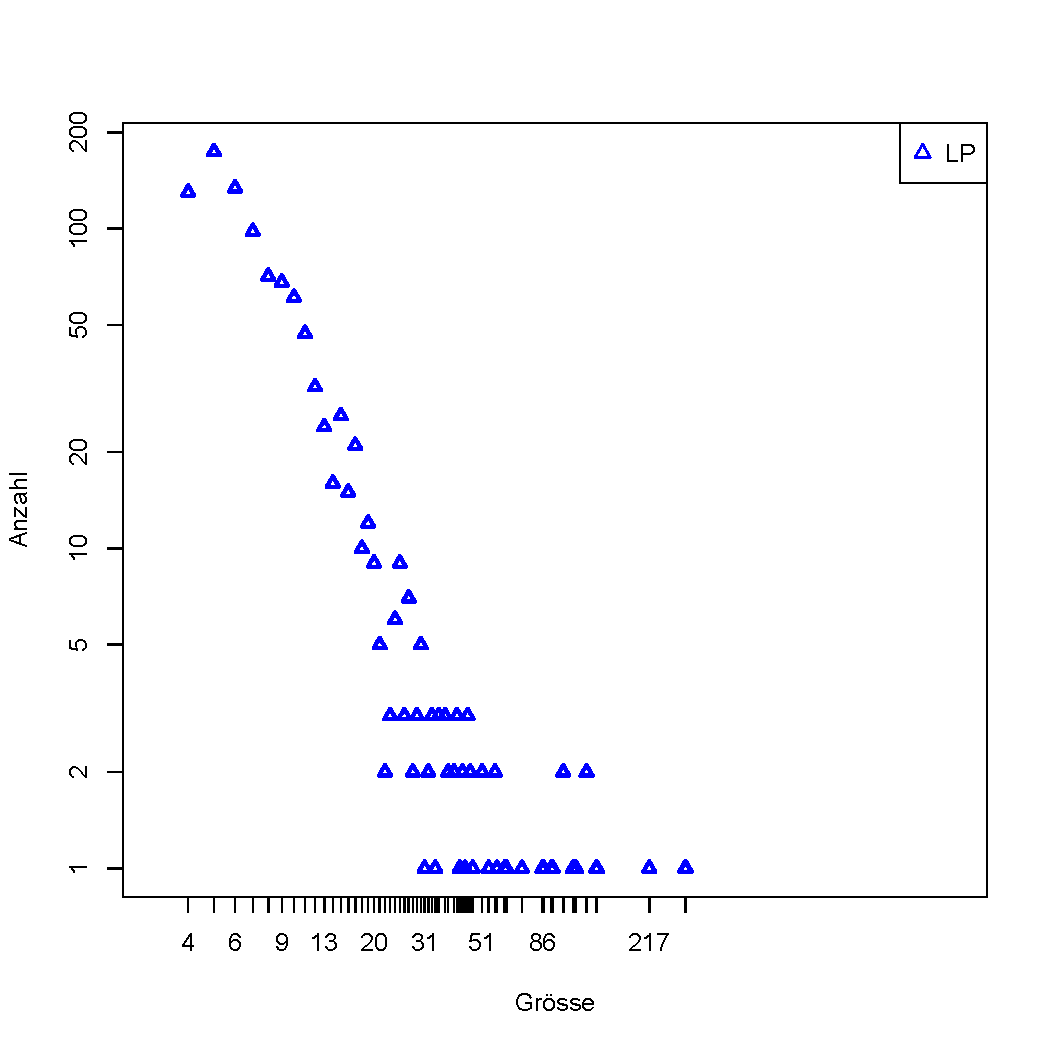
\includegraphics[scale=0.45]{images/tld-sure-ass_label.pdf}}
  \subfloat[]{\label{fig:comsize-bl2} 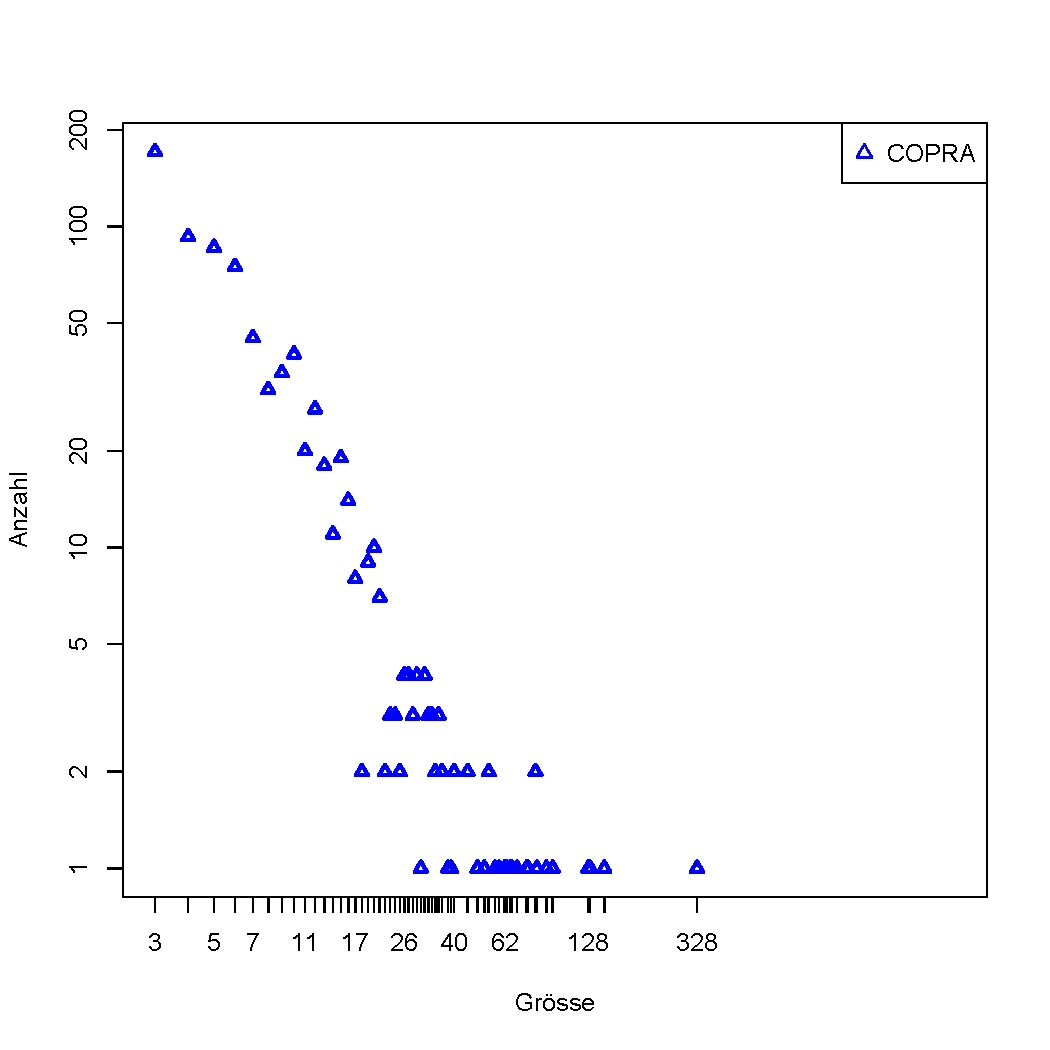
\includegraphics[scale=0.45]{images/tld-sure-ass_copra.pdf}}\\
  \subfloat[]{\label{fig:comsize-bl5} 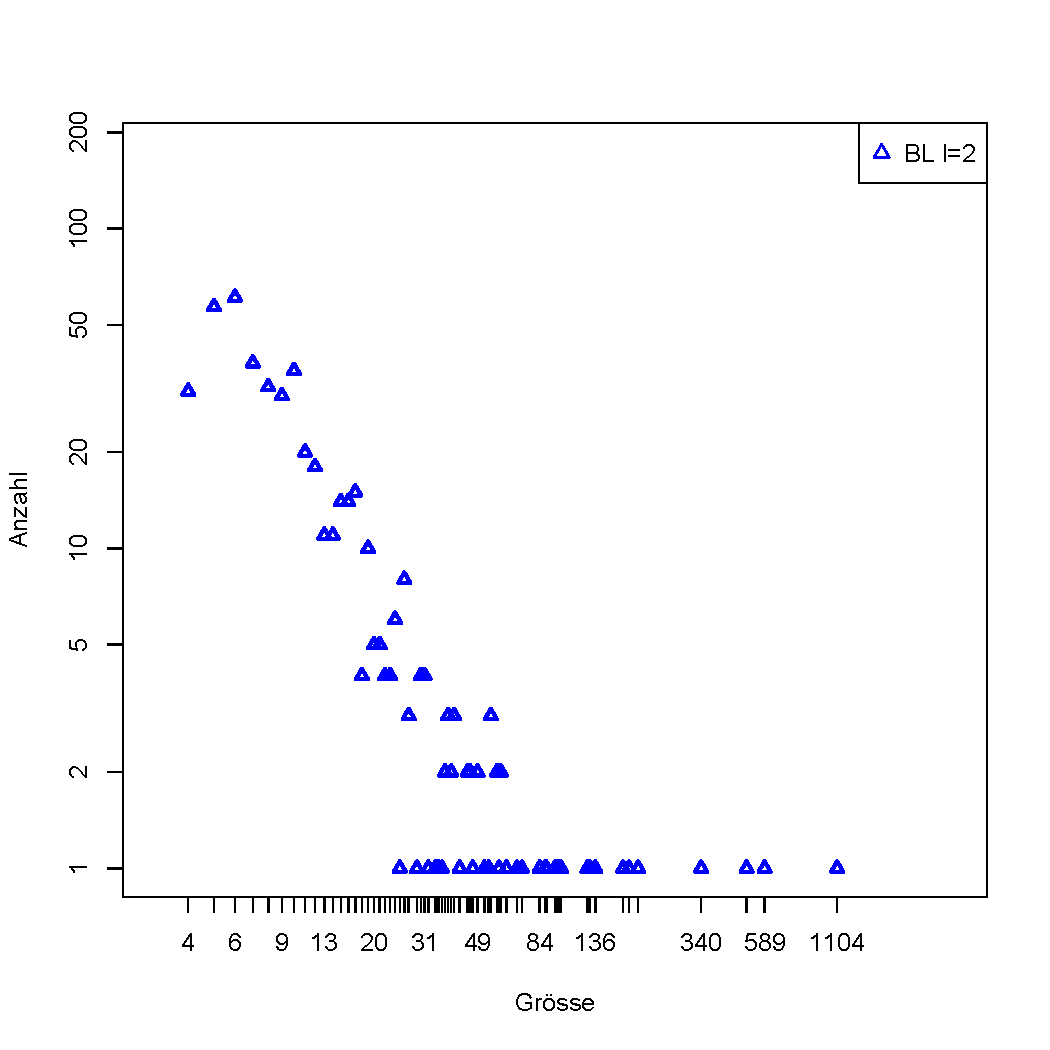
\includegraphics[scale=0.45]{images/tld-sure-ass_bl2.pdf}} 
  \subfloat[]{\label{fig:comsize-copra} 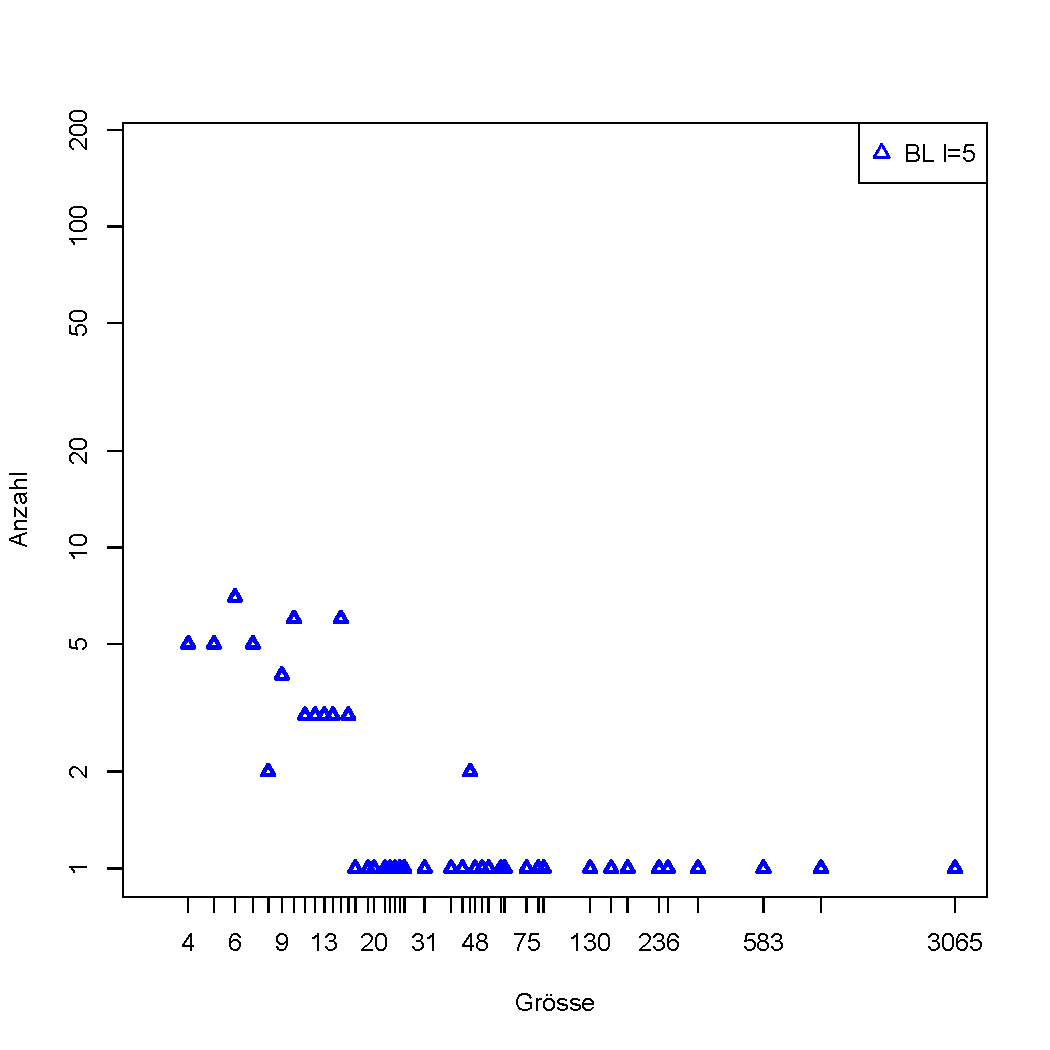
\includegraphics[scale=0.45]{images/tld-sure-ass_bl5.pdf}}
  \caption{Zuweisung von Domains zu TLDs abh\"angig von der Community-Gr\"osse}
  \label{fig:comsizedist}
\end{figure}

\begin{figure}[t]
  \centering
  \subfloat[]{\label{fig:comsize-lp} 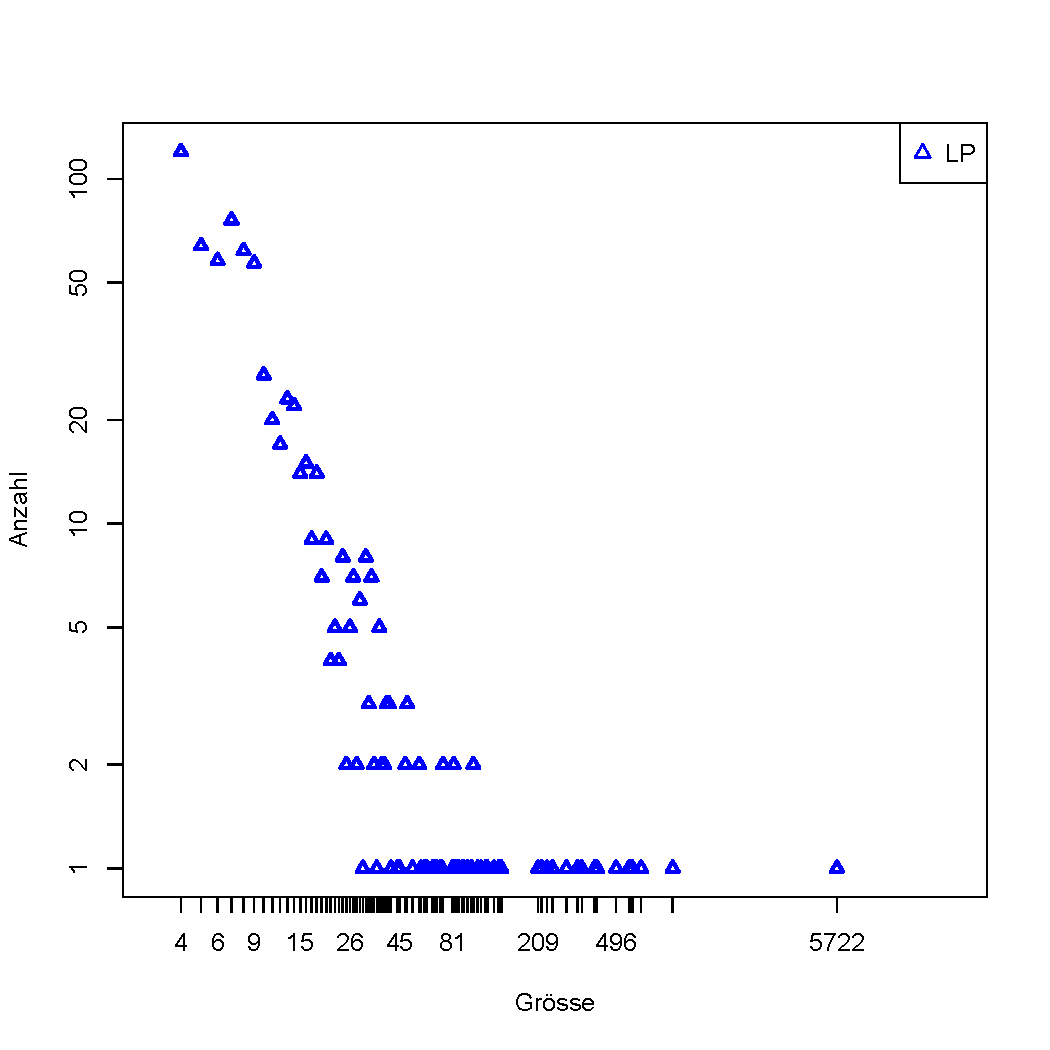
\includegraphics[scale=0.45]{images/tld-maybe-ass_label.pdf}}
  \subfloat[]{\label{fig:comsize-bl2} 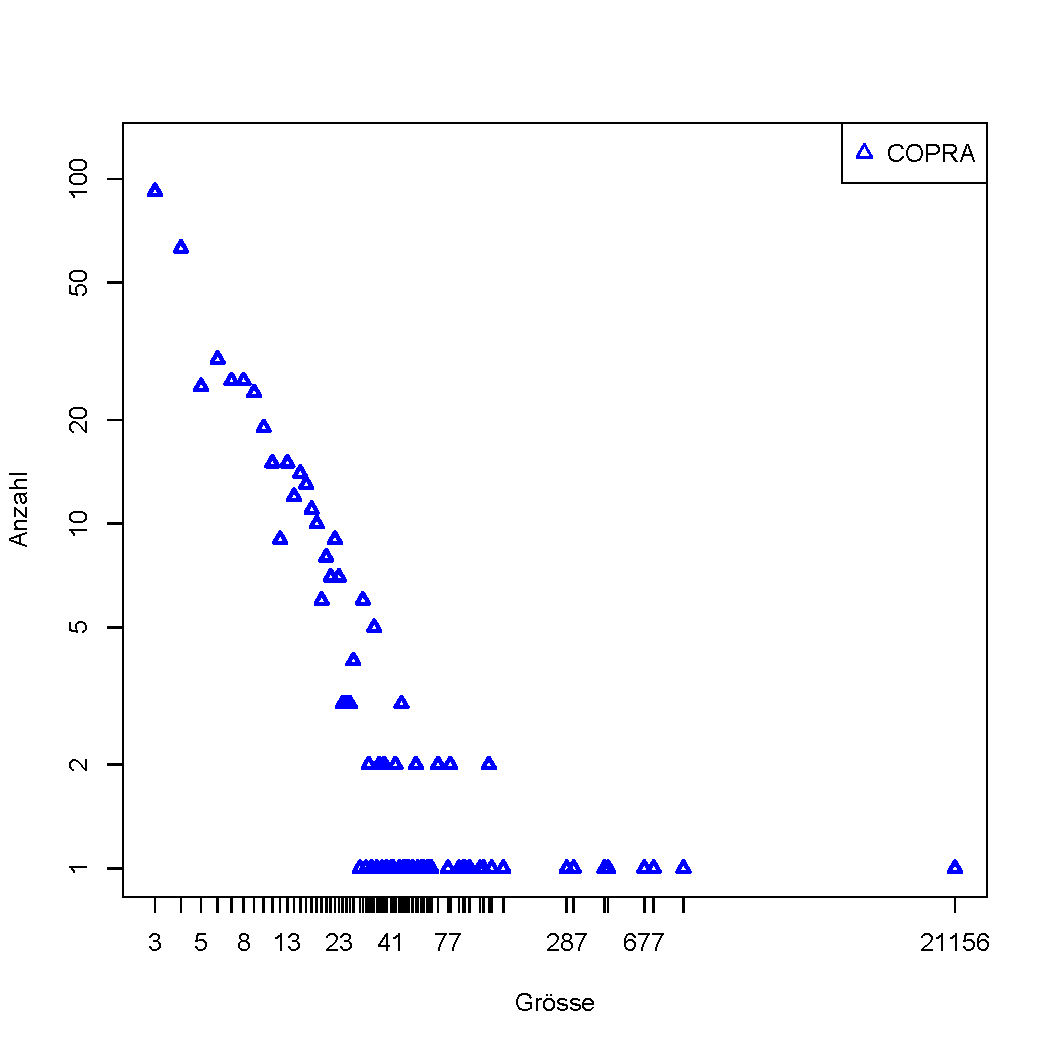
\includegraphics[scale=0.45]{images/tld-maybe-ass_copra.pdf}}\\
  \subfloat[]{\label{fig:comsize-bl5} 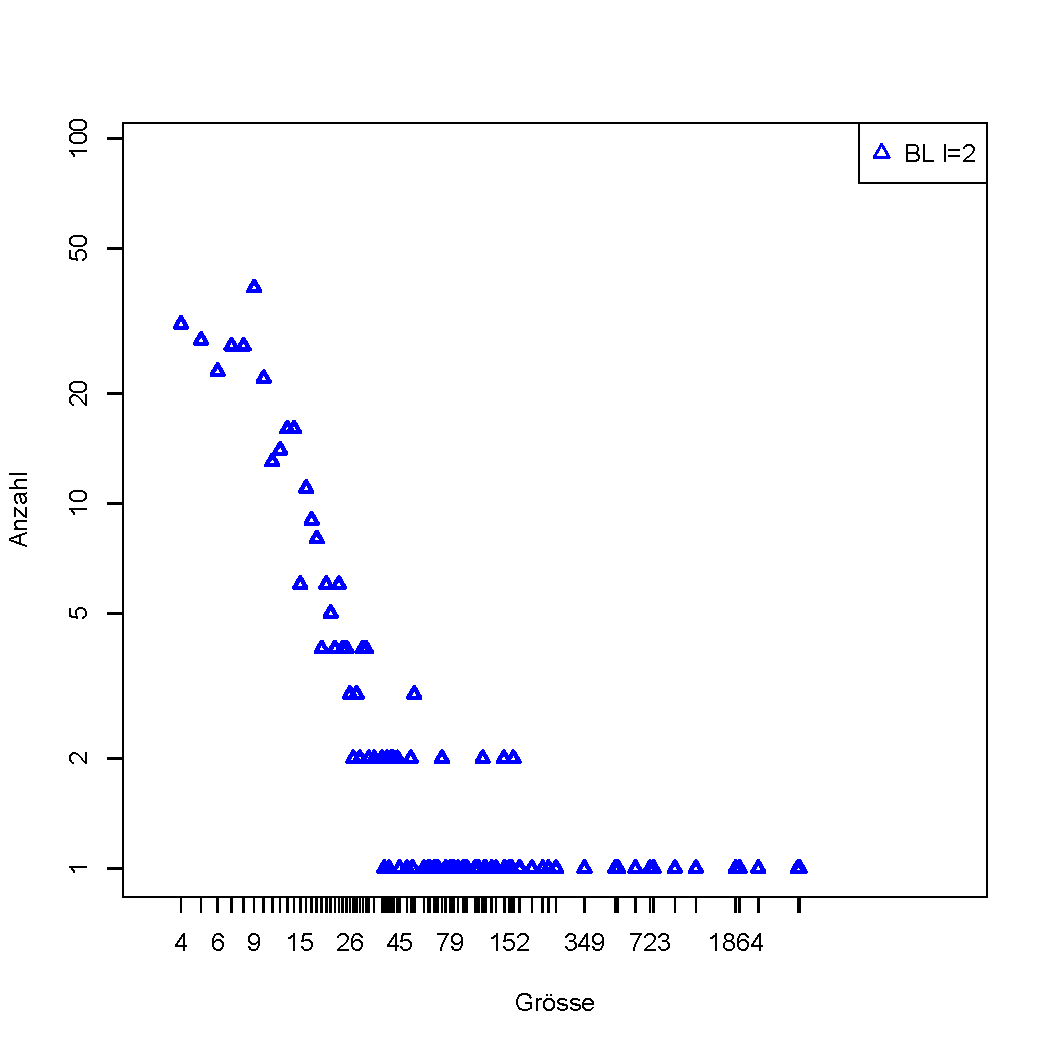
\includegraphics[scale=0.45]{images/tld-maybe-ass_bl2.pdf}} 
  \subfloat[]{\label{fig:comsize-copra} 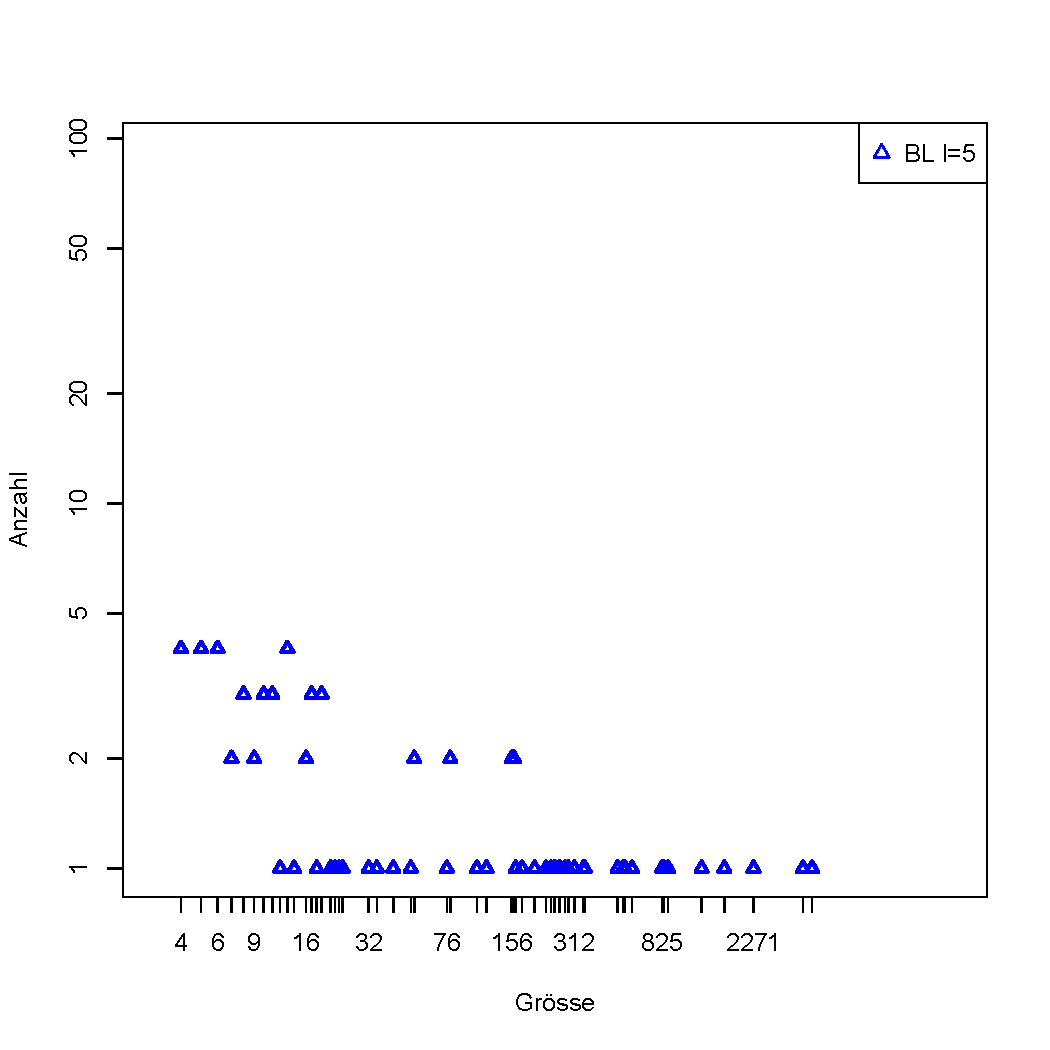
\includegraphics[scale=0.45]{images/tld-maybe-ass_bl5.pdf}}
  \caption{Verteilung der Gr\"osse der von einer TLD dominierten Communities}
  \label{fig:comsizedist}
\end{figure}

\begin{figure}[t]
  \centering
  \subfloat[]{\label{fig:comsize-lp} 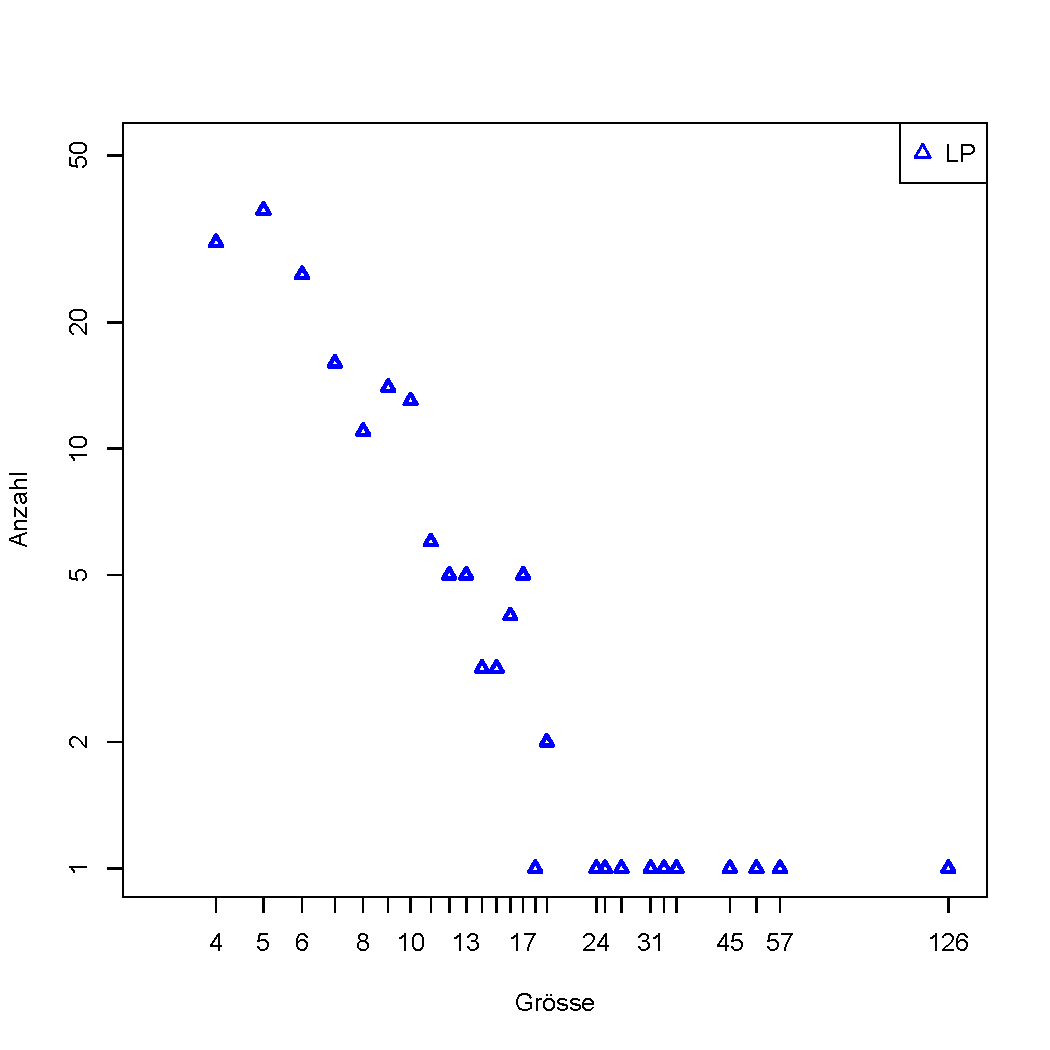
\includegraphics[scale=0.45]{images/sld-sure-ass_label.pdf}}
  \subfloat[]{\label{fig:comsize-bl2} 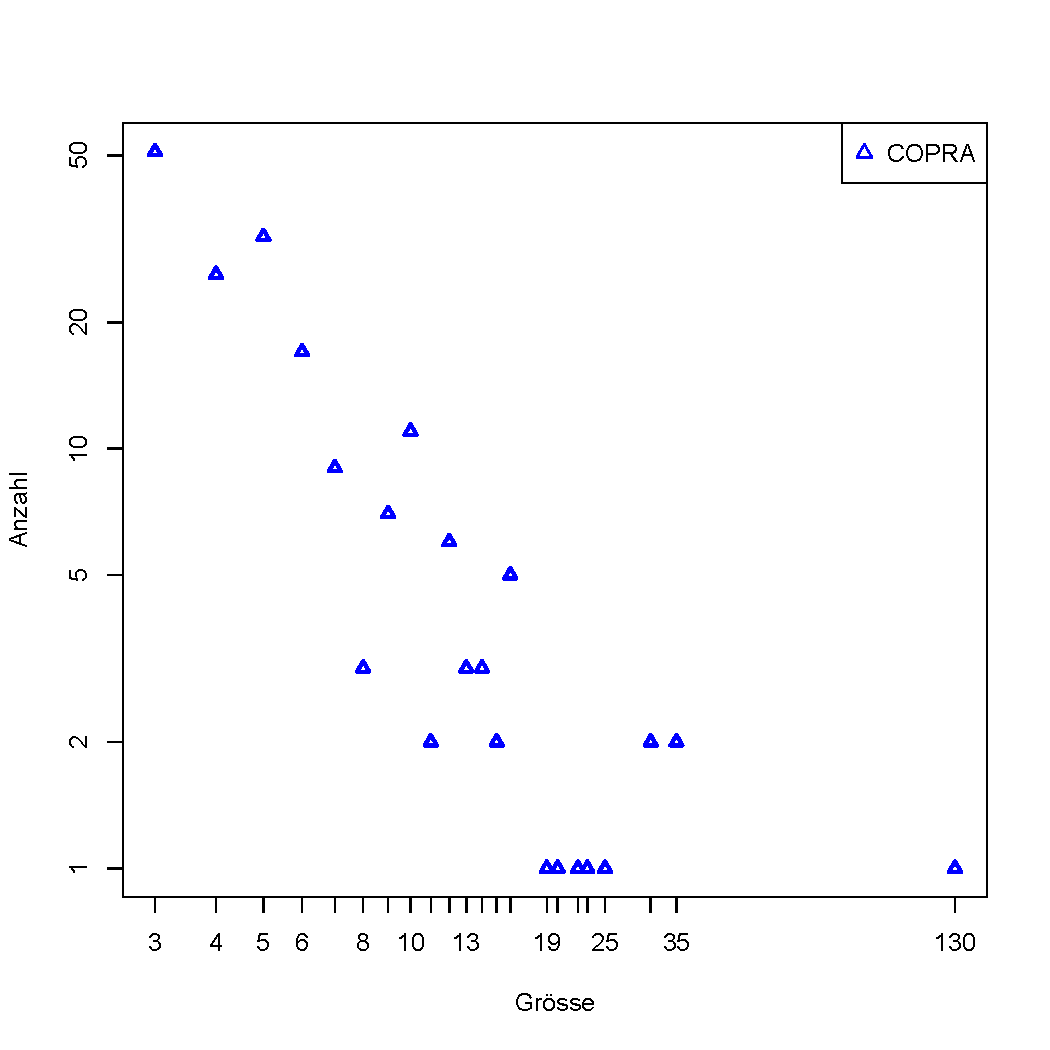
\includegraphics[scale=0.45]{images/sld-sure-ass_copra.pdf}}\\
  \subfloat[]{\label{fig:comsize-bl5} 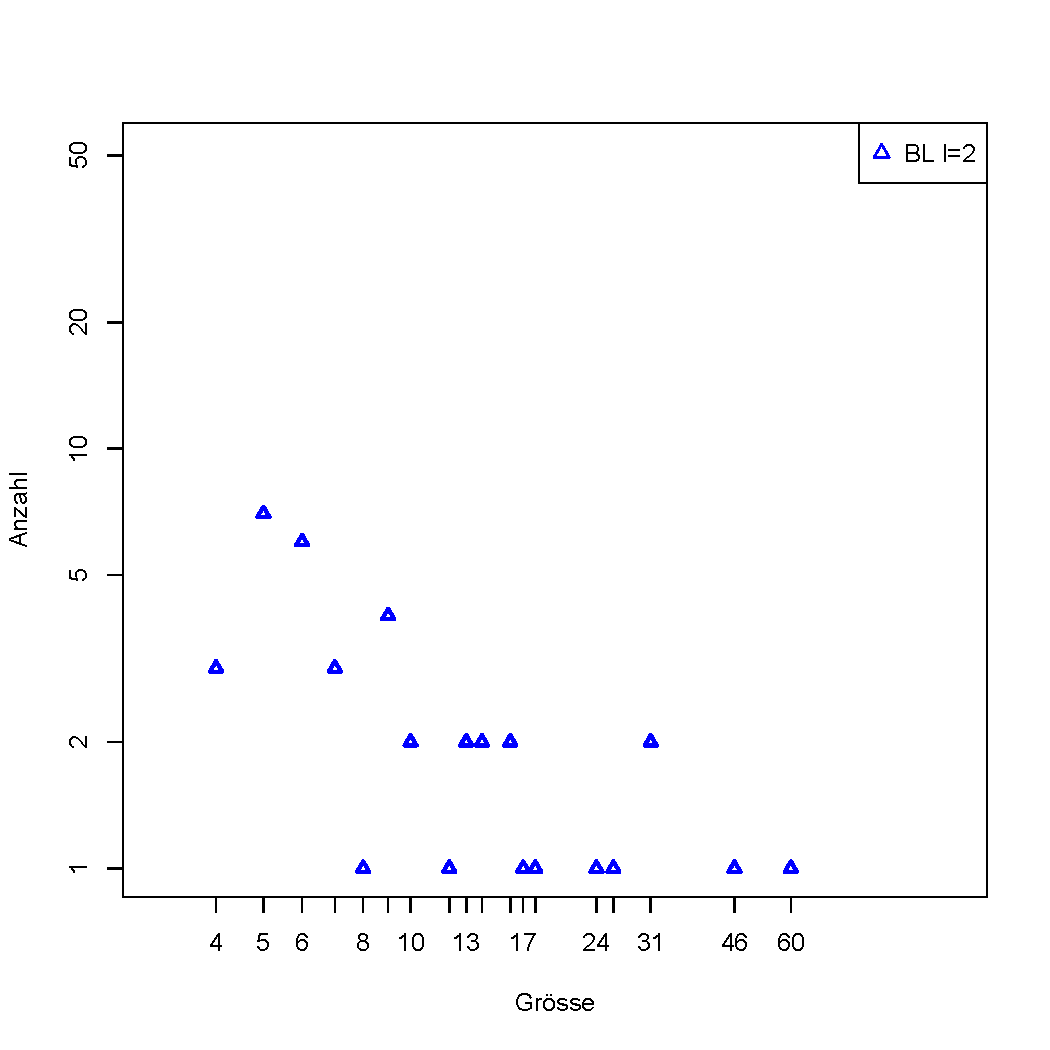
\includegraphics[scale=0.45]{images/sld-sure-ass_bl2.pdf}} 
  \subfloat[]{\label{fig:comsize-copra} 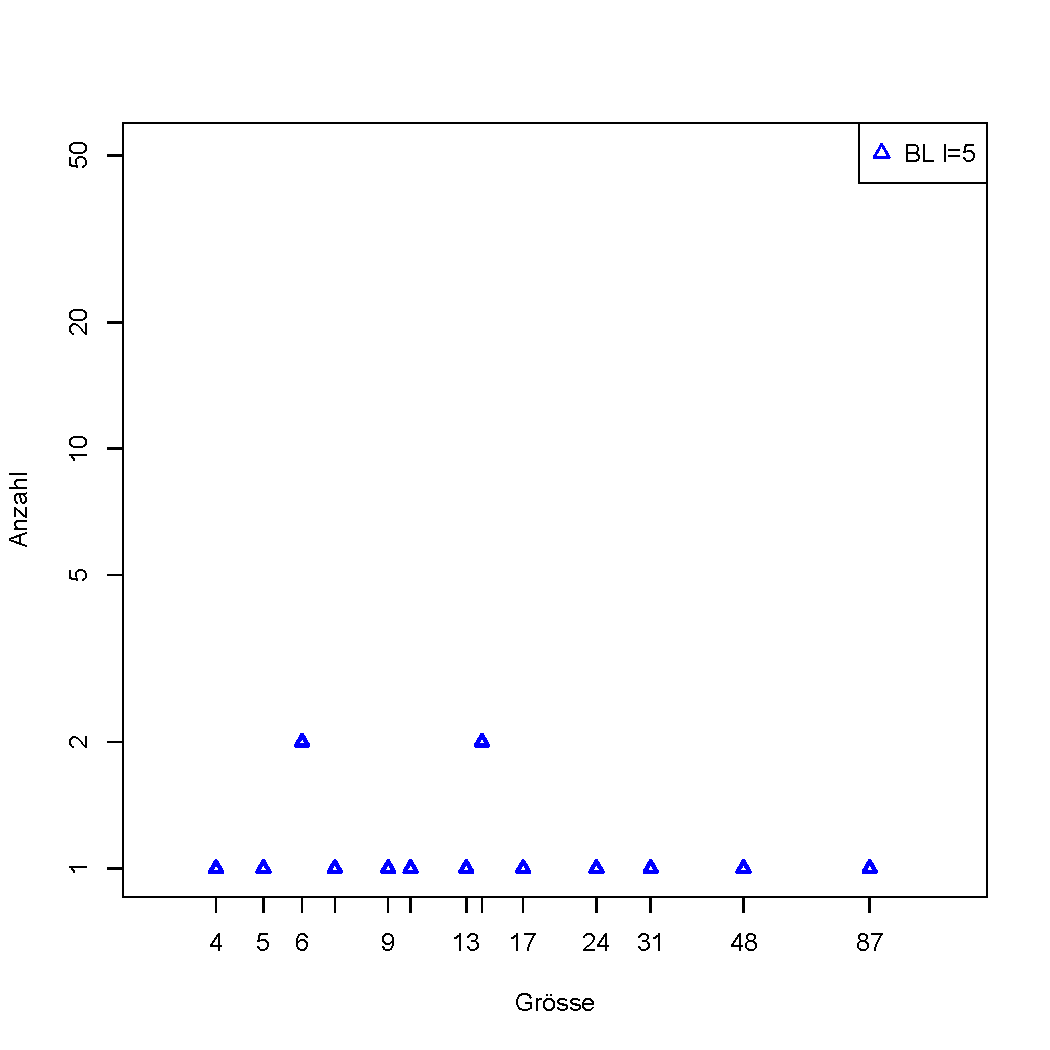
\includegraphics[scale=0.45]{images/sld-sure-ass_bl5.pdf}}
  \caption{Zuweisung von Domains zu SLDs abh\"angig von der Community-Gr\"osse}
  \label{fig:comsizedist}
\end{figure}

\begin{figure}[t]
  \centering
  \subfloat[]{\label{fig:comsize-lp} 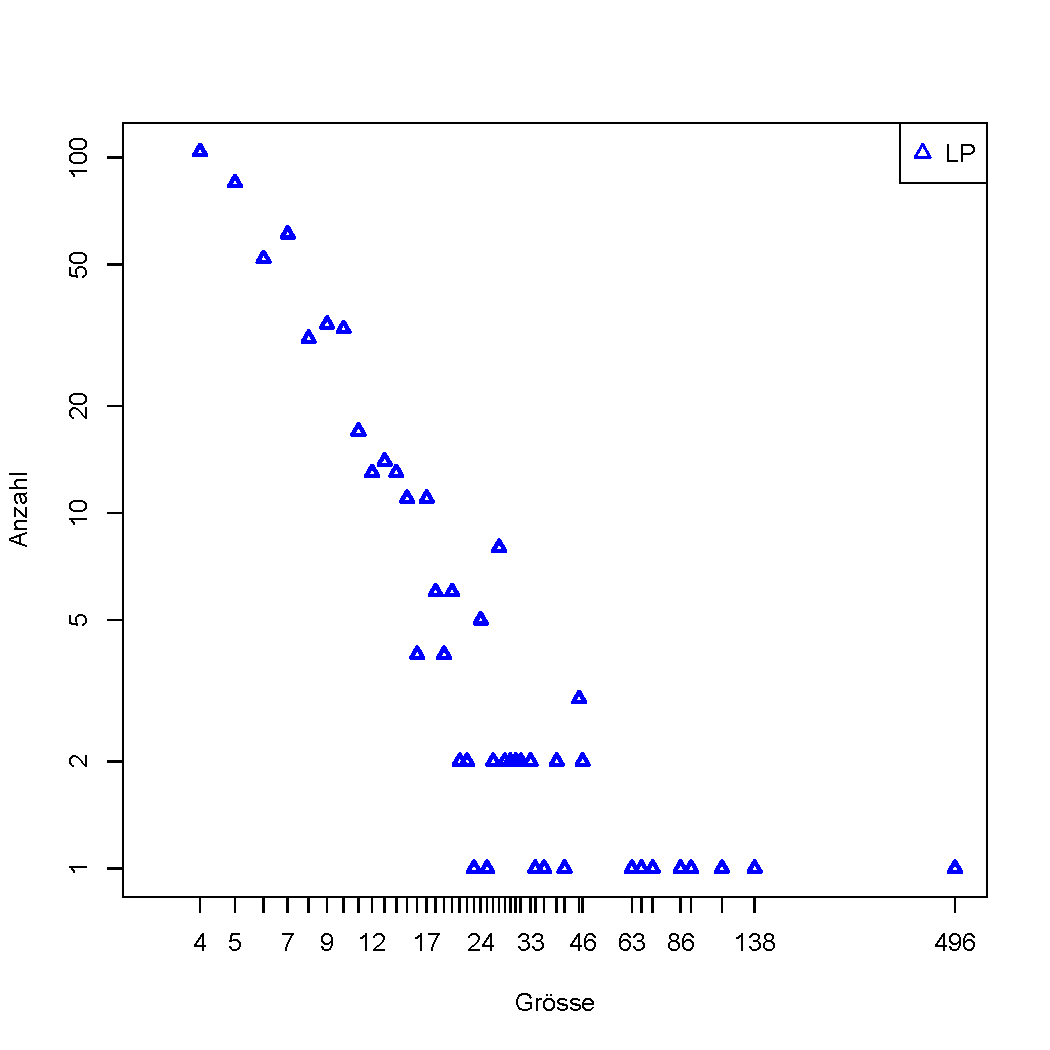
\includegraphics[scale=0.45]{images/sld-maybe-ass_label.pdf}}
  \subfloat[]{\label{fig:comsize-bl2} 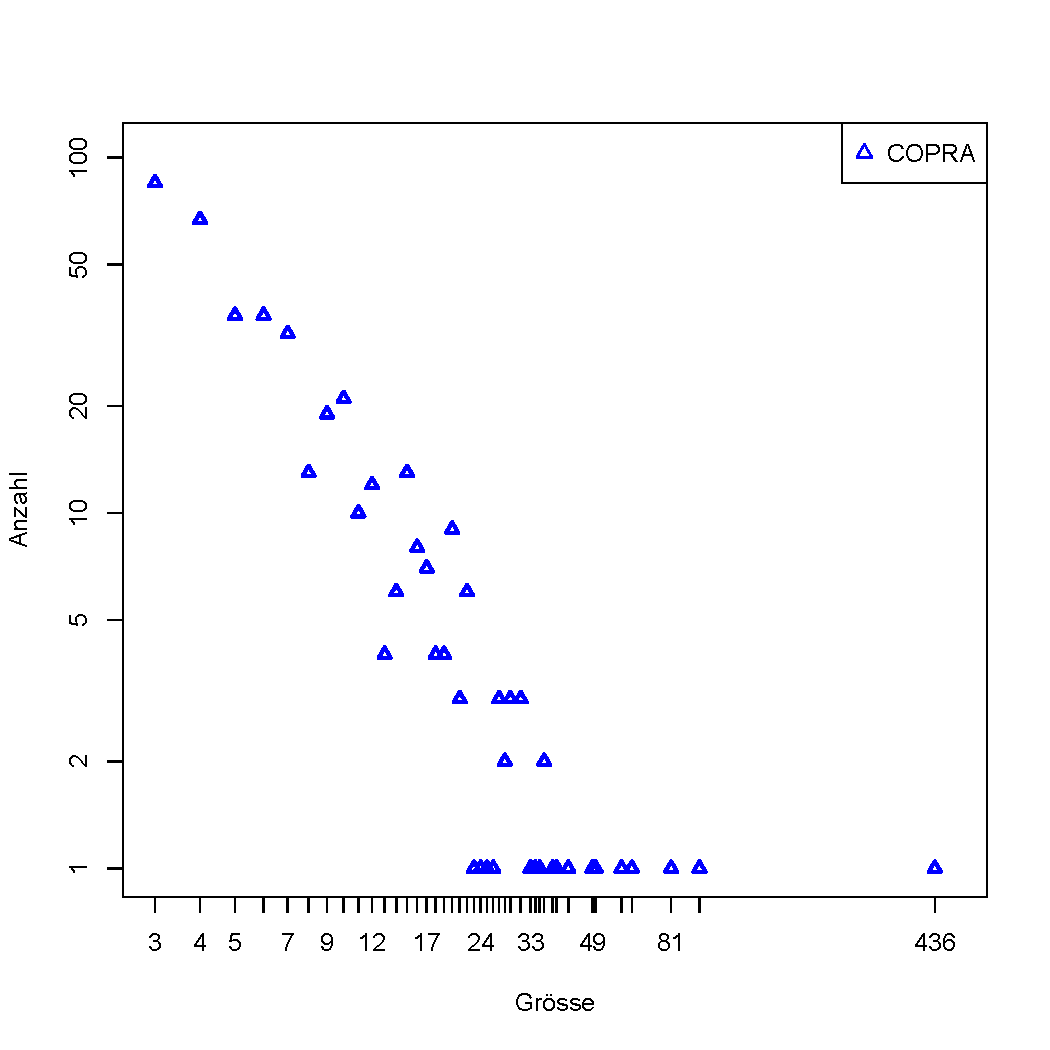
\includegraphics[scale=0.45]{images/sld-maybe-ass_copra.pdf}}\\
  \subfloat[]{\label{fig:comsize-bl5} 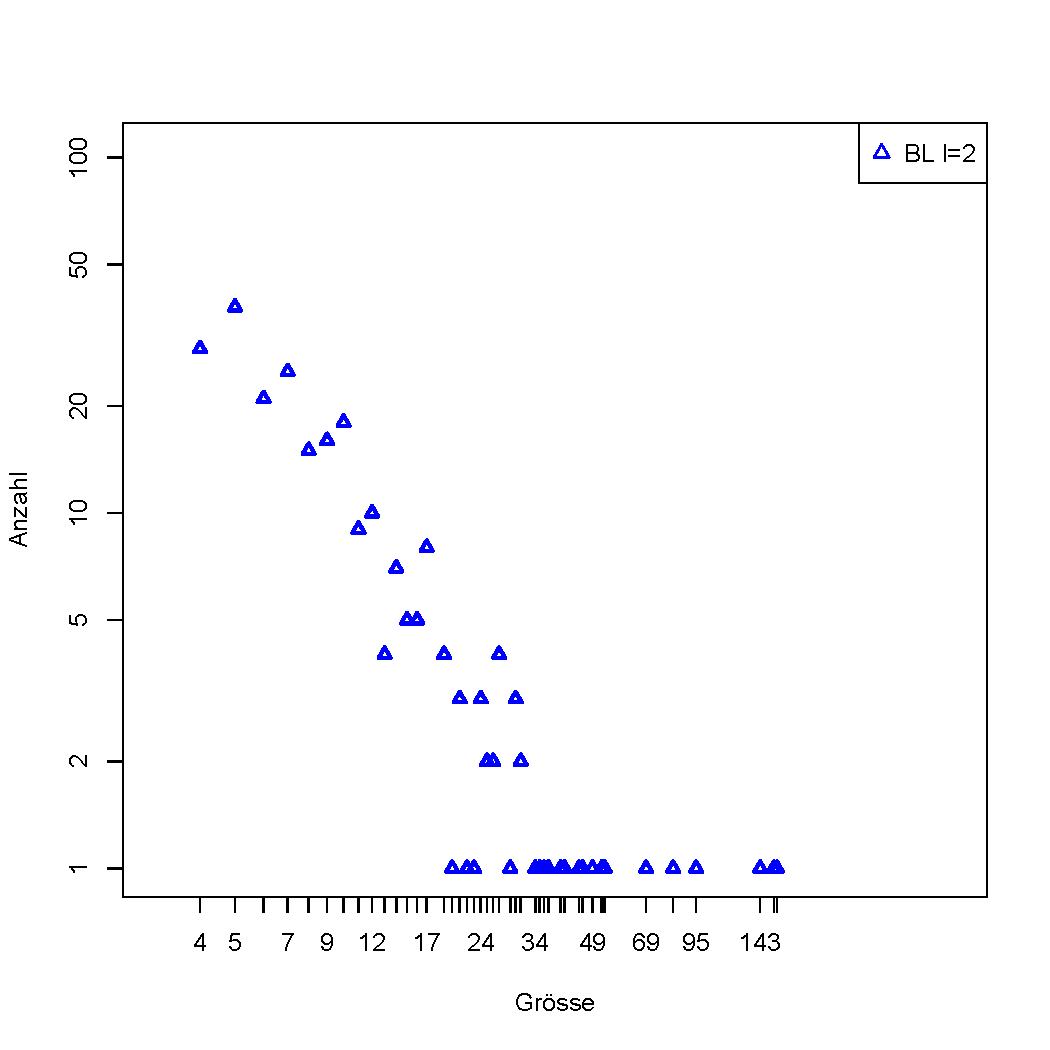
\includegraphics[scale=0.45]{images/sld-maybe-ass_bl2.pdf}} 
  \subfloat[]{\label{fig:comsize-copra} 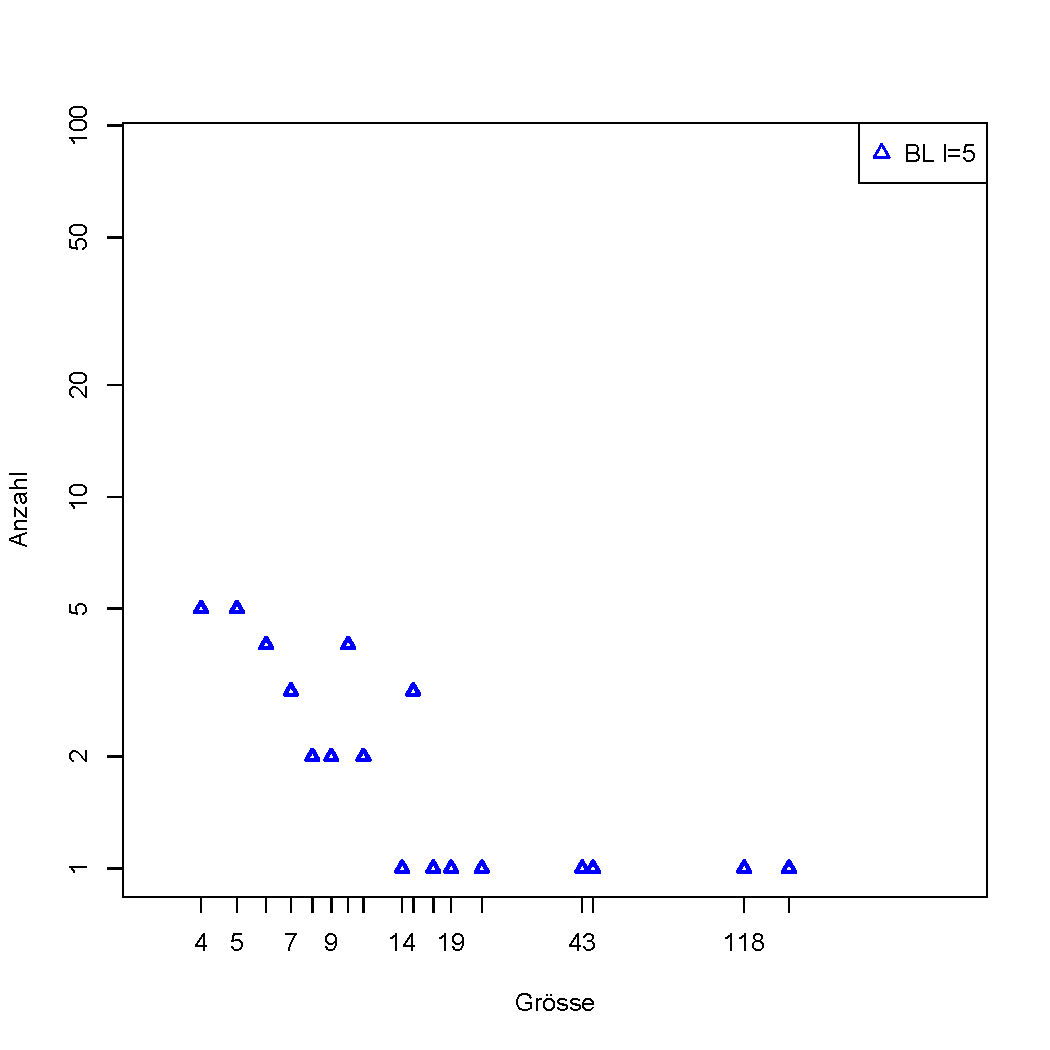
\includegraphics[scale=0.45]{images/sld-maybe-ass_bl5.pdf}}
  \caption{Verteilung der Gr\"osse der von einer SLD dominierten Communities}
  \label{fig:comsizedist}
\end{figure}

\begin{figure}[t]
  \centering
  \subfloat[]{\label{fig:comsize-lp} 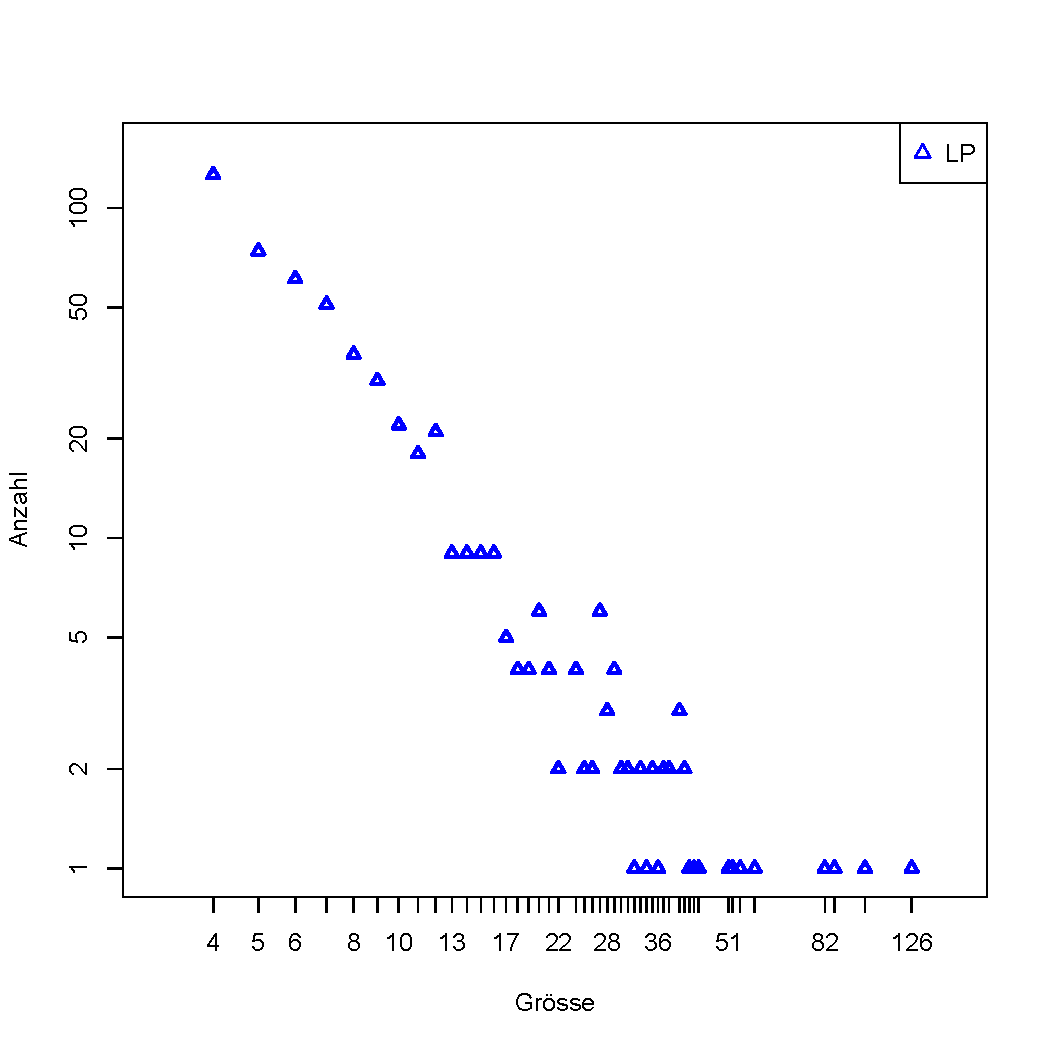
\includegraphics[scale=0.45]{images/time-corr_label.pdf}}
  \subfloat[]{\label{fig:comsize-bl2} 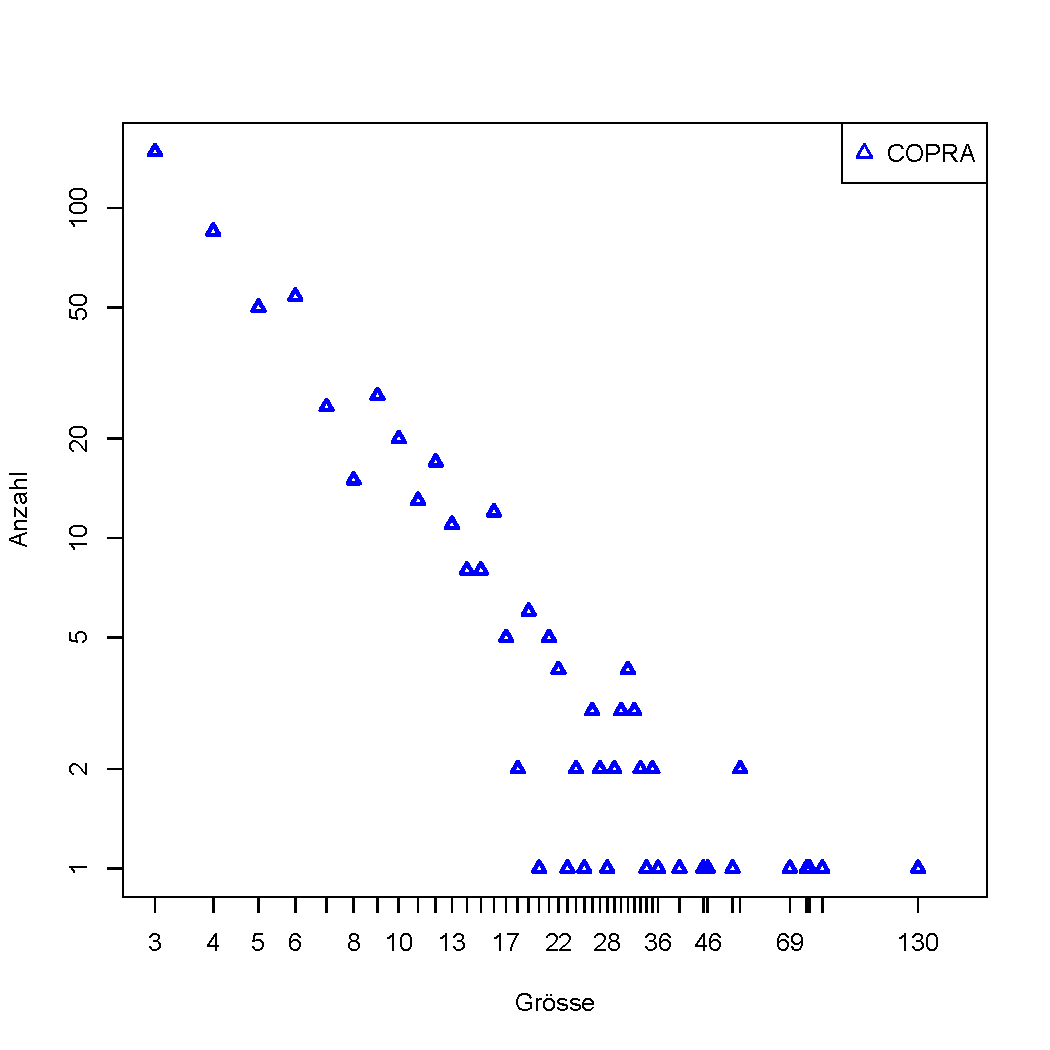
\includegraphics[scale=0.45]{images/time-corr_copra.pdf}}\\
  \subfloat[]{\label{fig:comsize-bl5} 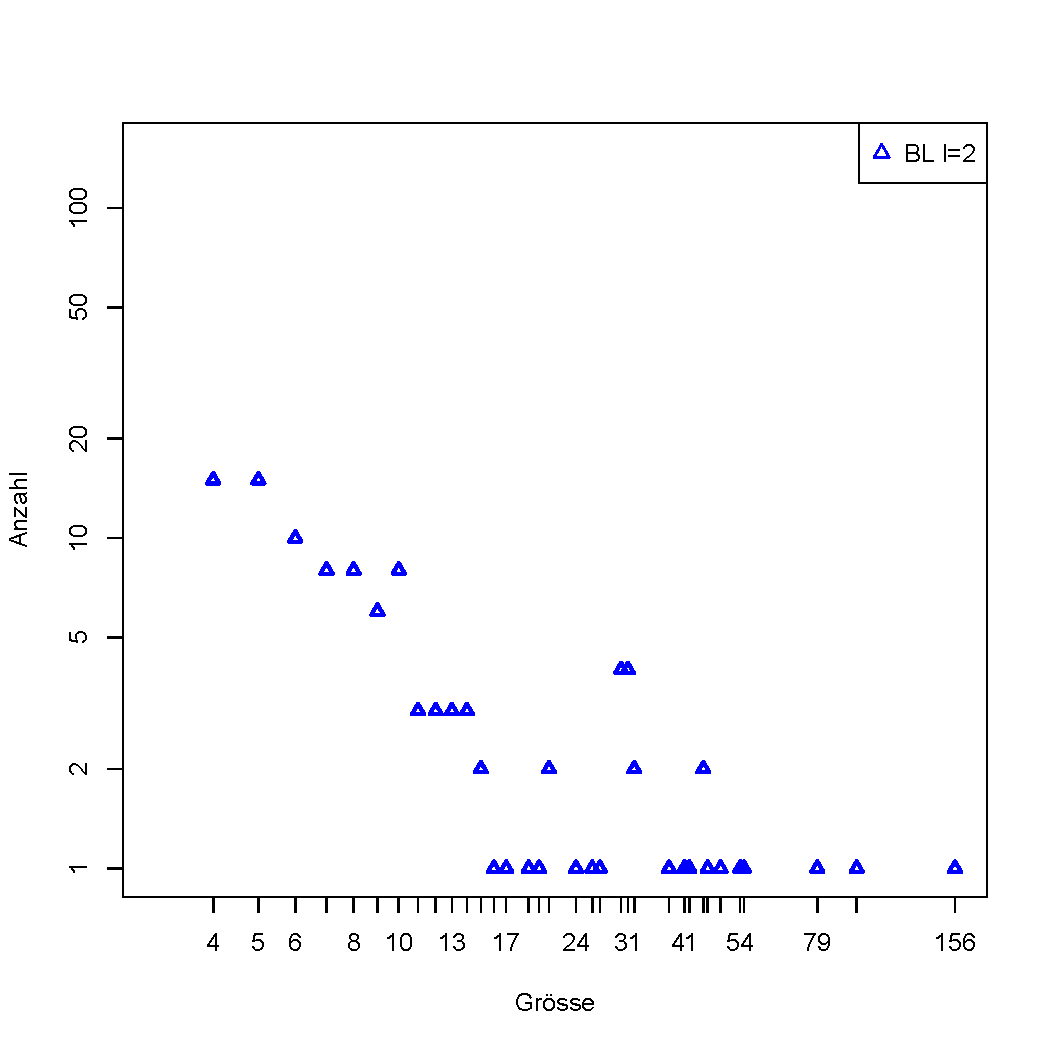
\includegraphics[scale=0.45]{images/time-corr_bl2.pdf}} 
  \subfloat[]{\label{fig:comsize-copra} 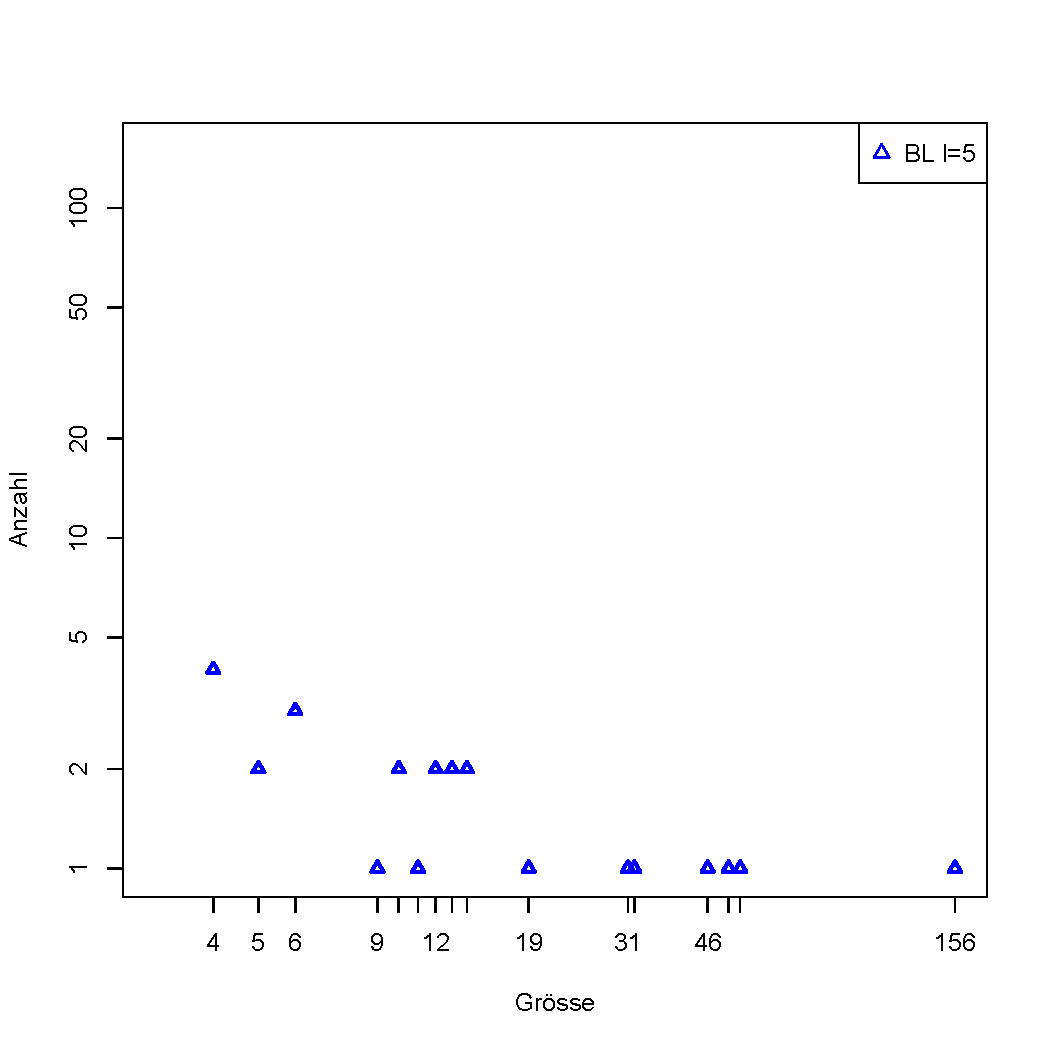
\includegraphics[scale=0.45]{images/time-corr_bl5.pdf}}
  \caption{Verteilung der Gr\"osse von Communities mit zeitlicher
    Korrelation der Signaturen}
  \label{fig:comsizedist}
\end{figure}

erichteten Graphen definiert. Ebenso 

%%% Local Variables: 
%%% mode: latex
%%% TeX-master: "diplarb"
%%% End: 
